\documentclass{isrmdelo}

%-----------------------------------------------------------------------------
%   Podatki o delu
%-----------------------------------------------------------------------------

\avtor{Adrijan Rogan}

\naslov{Kaos v diskretnih dinamičnih sistemih}
\title{Chaos in discrete dynamical systems}

\mentor{}
\mentorica{prof. dr. Barbara Drinovec Drnovšek}
\somentor{doc. dr. Luka Boc Thaler}
\somentorica{}

\letnica{2022}

\opis{Študent uvede diskretne dinamične sisteme in lastnosti, ki definirajo kaotične dinamične sisteme. Nato se posveti šotorski preslikavi in obravnava njeno dinamiko.}
\desc{The student introduces discrete dynamical systems and the properties that define chaotic dynamical systems. Then he studies the tent mapping and discusses its dynamics.}

\povzetek{V delu raziščemo kaos v diskretnih dinamičnih sistemih. Najprej definiramo splošne dinamične sisteme in vpeljemo iteracijo preslikave kot klasični zgled diskretnega dinamičnega sistema. Opišemo tri zahteve, ki določajo kaotične diskretne dinamične sisteme: občutljivost na začetne pogoje, gostost periodičnih točk in topološka tranzitivnost. Ogledamo si družino šotorskih preslikav $T_\mu$ v odvisnosti od parametra $\mu > 0$ in raziščemo njihovo dinamiko. Pri določenih parametrih $\mu$ je dinamični sistem, porojen z iteriranjem preslikave $T_\mu$, kaotičen. Za parameter $\mu = 2$ dokažemo, da sistem zadošča zahtevam kaotičnih dinamičnih sistemov. Za parametre $\mu > 2$ vpeljemo simbolni prostor $\Sigma_2$ in pokažemo, da je pomik $\sigma$ kaotična preslikava. Nato definiramo preslikavo, ki je topološka konjugacija med $T_\mu$ in $\sigma$ in pokažemo, da ohranja kaotičnost.}

\abstract{In this diploma thesis, we explore chaos in discrete dynamical systems. First, we define dynamical systems in general and introduce an iterated map as the prototypical example of a discrete dynamical system. We describe the three conditions that define chaotic discrete dynamical systems: sensitive dependence on initial conditions, dense periodic points and topological transitivity. Then, we examine the dynamics of the one-parameter family of tent maps $T_\mu$ where $\mu > 0$ and show that the dynamic system arising from iterating $T_\mu$ is chaotic for some parameters $\mu$. For $\mu = 2$, we directly check that the system meets criteria for chaotic systems. For $\mu > 2$, we introduce the symbol space $\Sigma_2$ and show that the shift map $\sigma$ is chaotic. We then define a map that is a topological conjugacy between $T_\mu$ and $\sigma$ and show that it preserves chaoticity.}

% navedite vsaj eno klasifikacijsko oznako --
% dostopne so na www.ams.org/mathscinet/msc/msc2010.html
\klasifikacija{26A18, 37B10, 37E05}
\kljucnebesede{diskretni dinamični sistem, kaos, šotorska preslikava, Cantorjeva množica, topološka konjugacija, simbolna dinamika} % navedite nekaj ključnih pojmov, ki nastopajo v delu
\keywords{discrete dynamical system, chaos, tent map, Cantor set, topological conjugation, symbolic dynamics} % angleški prevod ključnih besed

%-----------------------------------------------------------------------------
%   Paketi, definicije itd.
%-----------------------------------------------------------------------------

% poskrbi za metapodatke in veljaven PDF/A-1b standard
\zapisiMetaPodatke

\usepackage[pdftex]{graphicx}

\usepackage{tikz}
\usepackage{tikz-cd}
\usetikzlibrary{arrows}

\usepackage{enumitem}
\setlist{itemsep=2pt,parsep=2pt,topsep=4pt}

\usepackage[sorting=nty]{biblatex}
\addbibresource{refs.bib}

\usepackage{braket}

\usepackage[autostyle=false, style=german]{csquotes}

% za številske množice uporabite naslednje simbole
\newcommand{\R}{\mathbb R}
\newcommand{\N}{\mathbb N}
\newcommand{\Z}{\mathbb Z}
\newcommand{\C}{\mathbb C}
\newcommand{\Q}{\mathbb Q}

% Oznaka za konstruirano Cantorjevo množico
\newcommand{\cantorset}{\mathcal{C}}

% Oznaka za identiteto (preslikava)
\newcommand{\id}{\mathrm{id}}

% slovenski narekovaji
\newcommand{\narekovaji}[1]{,,#1``}

\newcommand{\ignore}[1]{}

%-----------------------------------------------------------------------------
%   Dokument
%-----------------------------------------------------------------------------

\begin{document}

\chapter{Matematični kaos}

Teorija kaosa ima bogato matematično zgodovino. Opišimo nekaj ključnih trenutkov, kot jih navajata matematik Steve Smale v članku \cite{smale98} in pisatelj James Gleick v knjigi \cite{gleick}. Začetki teorije kaosa segajo v konec 19.\ stoletja, ko se je francoski matematik Henri Poincaré ukvarjal s problemom treh teles (dinamika gravitacijskih interakcij med nebesnimi telesi) in opazil, da je dolgoročno obnašanje težko napovedati in da stabilnost sistema ni zagotovljena.

Na zavedanje o obstoju kaotičnih sistemov, ki se porodijo iz fizikalnih modelov sveta, je pomembno vplival Edward Lorenz v šestdesetih letih 20.\ stoletja s svojim poenostavljenim modelom vremena, ki ga Gleick opisuje na začetku svoje knjige. Za svoje izračune je uporabljal računalnik, ki je števila predstavil s šestimi decimalnimi mesti, na papir pa so bili natisnjeni z le štirimi decimalnimi mesti. Ko je želel ponoviti neko simulacijo, je za začetne pogoje vnesel števila z natisnjenega papirja, pognal model in ugotovil, da se novi izračuni ne skladajo s starimi in da ta majhna sprememba na dolgi rok popolnoma spremeni stanje sistema, kot kaže slika \ref{fig:lorenz}. Temu pojavu pravimo \emph{metuljev učinek} (ang. butterfly effect) in je ena izmed temeljnih lastnosti kaosa, ki ga bomo kasneje natančno definirali.

\begin{figure}[h!]
\begin{center}
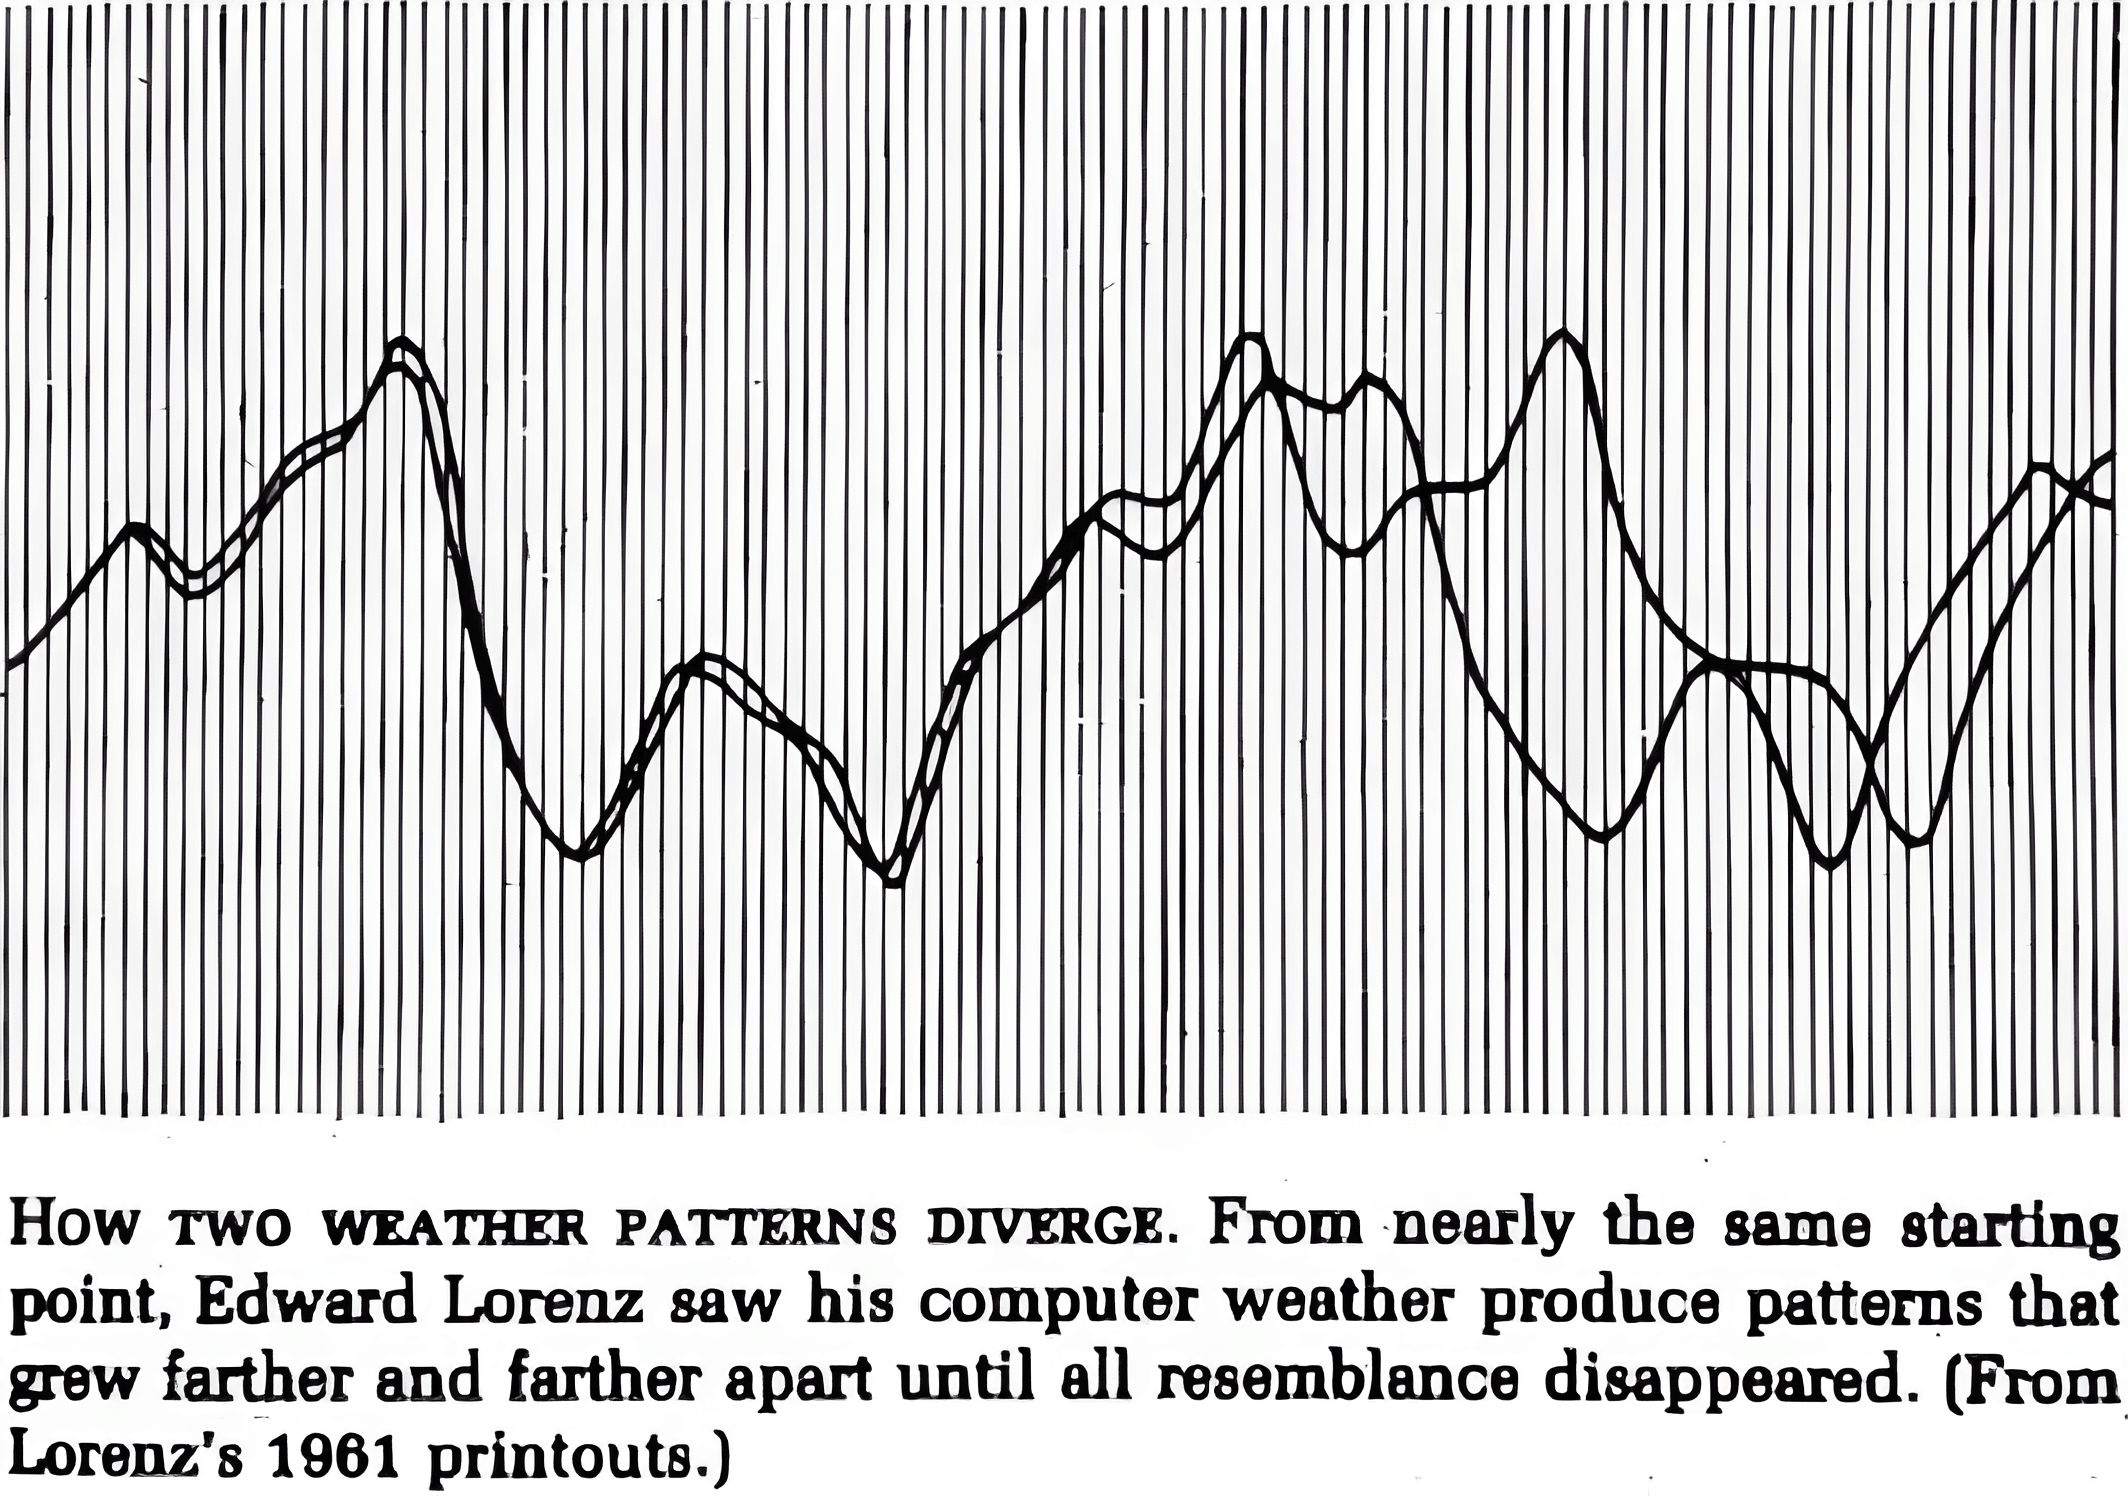
\includegraphics[width=0.6\textwidth]{img/lorenz_vreme.jpg}
\end{center}
\caption{Divergenca pri napovedi vremena ob majhni spremembi začetnih pogojev, vir: \cite{gleick}, stran 17}
\label{fig:lorenz}
\end{figure}

Stephen Smale, ki dogajanje z lastnimi besedami opiše v \cite{smale98}, je v tem času delal kot postdoktorski raziskovalec v Riu v Braziliji in v svojem članku postavil domnevo, ki je imela za posledico zanikanje obstoja kaosa. Kmalu za tem je Norman Levinson v pismu Smaleu pisal o svojih rezultatih, ki so nasprotovali njegovi domnevi. Pojasnjeval je obsežno delo britanskih matematikov Mary Cartwright in Johna Edensorja Littlewooda, ki sta med drugo svetovno vojno proučevala Van der Polovo nihalo. Analiza nihala s strani Cartwright, Littlewooda in Levinsona je Smalea vodila v razvoj podkvaste preslikave, ki je imela kaotično obnašanje nihala, ampak je bila enostavnejša. Danes je znano, da se Smaleova podkev pojavlja v mnogih dinamičnih sistemih. V tem delu bomo analizirali njeno poenostavitev na enodimenzionalni prostor.

\section{Metrični prostor}

\begin{definicija}
Naj bo $X$ množica in $d: X \times X \rightarrow \R$ preslikava, za katero velja:
\begin{enumerate}
\item $d(x,y) = 0 \iff x = y \quad \forall x,y \in X$,
\item $d(x,y) = d(y,x) \quad \forall x,y \in X$ (\emph{simetričnost}) in
\item $d(x,y) \leq d(x,z) + d(z,y) \quad \forall x,y,z \in X$ (\emph{trikotniška neenakost}).
\end{enumerate}
Potem paru $(X, d)$ pravimo \emph{metrični prostor}, preslikavi $d$ pa \emph{metrika na $X$}.
\end{definicija}

\medskip

Zgornje lastnosti zagotavljajo, da je $d(x,y) \geq 0$. Namreč, po trikotniški neekosti velja $d(x,y) + d(y,x) \geq d(x,x)$, torej je po prvi in drugi lastnosti $2d(x,y) \geq 0$, zato je $d(x,y) \geq 0$.

\bigskip

\begin{definicija}
Naj bo $(X,d)$ metrični prostor. \emph{Odprta krogla} s središčem v $x$ in polmerom $r$ je množica $$K_r(x) = \set{ y \in X \mid d(x,y) < r }.$$
\end{definicija}

Na sliki \ref{fig:krogle} so prikazane odprte krogle v treh metričnih prostorih. Prvi je običajen prostor realnih števil z metriko $d(x,y) = \vert x-y \vert$, drugi je $\R^2$ z običajno evklidsko metriko $d(x,y) = \sqrt{(x_1-x_2)^2 + (y_1-y_2)^2}$, in tretji je $\R^2$ z metriko $d(x,y) = \max \set{ \vert x_1-x_2 \vert, \vert y_1-y_2 \vert }$.

\begin{figure}[h!]  
\centering 
\begin{tikzpicture}

\draw[-, thick, gray] (0,1) -- (2,1);
\draw[(-), thick] (0.4,1) -- (1.6,1);
\fill (1,1) circle[radius=1pt] node[below]{$x$};

\draw[-, thick] (4,0) -- (6,0);
\draw[-, thick] (4,0) -- (4,2);
\fill (4.8,0.9) circle[radius=1pt] node[below]{$x$};
\draw[dashed] (4.8,0.9) circle[radius=1];

\draw[-, thick] (8,0) -- (10,0);
\draw[-, thick] (8,0) -- (8,2);
\fill (8.8,0.7) circle[radius=1pt] node[below]{$x$};
\draw[dashed] (8.8,0.7) +(-0.5,-0.5) rectangle +(0.5,0.5);

\end{tikzpicture}
\bigskip
\caption{Odprte krogle v raznih metričnih prostorih} \label{fig:krogle}  
\end{figure} 

\begin{opomba}
Odprti krogli s polmerom $\varepsilon$ in središčem v $x$ včasih pravimo tudi \emph{$\varepsilon$-okolica točke $x$}.
\end{opomba}

\begin{definicija}
Naj bo $(X,d)$ metrični prostor. Podmnožica $A \subseteq X$ je \emph{odprta}, če za vsak $a \in A$ obstaja $r > 0$, tako da je krogla $K_r(a)$ popolnoma vsebovana v $A$.
\end{definicija}

\begin{trditev}
Odprta krogla je odprta množica v vsakem metričnem prostoru.
\end{trditev}

\begin{dokaz}
Vzemimo odprto kroglo $K_r(x)$. Pokazati želimo, da za vsak $y$ iz krogle $K_r(x)$ obstaja neka krogla $K_{r'}(y)$, tako da $K_{r'}(y) \subseteq K_r(x)$. Naj bo $0 < r' \leq r - d(x,y).$ Potem je $K_{r'}(y) \subseteq K_r(x)$, saj za vsak $z \in K_{r'}(y)$ velja 
\begin{equation*}
d(x,z) \leq d(x,y) + d(y,z) < d(x,y) + r' \leq r. \qedhere
\end{equation*}
\end{dokaz}

\begin{trditev}
\label{trditev:metrika_unija}
Unija poljubne družine odprtih množic je odprta množica v vsakem metričnem prostoru.
\end{trditev}

\begin{dokaz}
Naj bo $\set{U_i}_{i \in \mathcal{I}}$ poljubna družina odprtih množic in izberimo neko točko $x$ iz unije $\bigcup_{i \in \mathcal{I}} U_i$. Potem je $x \in U_j$ za nek $j \in \mathcal{I}$. Ker je $U_j$ odprta, obstaja krogla $K_r(x) \subseteq U_j$. Potem velja tudi $K_r(x) \subseteq \bigcup_{i \in \mathcal{I}} U_i$. \qedhere
\end{dokaz}

\begin{trditev}
\label{trditev:metrika_presek}
Presek končne družine odprtih množic je odprta množica v vsakem metričnem prostoru.
\end{trditev}

\begin{dokaz}
Naj bodo $U_1, U_2, \dots, U_n$ vse množice iz družine odprtih množic in vzemimo poljuben $x \in \bigcap_{i=1}^{n} U_i$. Potem je $x \in U_i$ za vsak $1 \leq i \leq n$ in ker so vse množice $U_i$ odprte, obstajajo krogle $K_{r_i}(x) \subseteq U_i$. Naj bo $r = \min \set{r_1, \dots, r_n}$. Potem je $K_r(x) \subseteq K_{r_i}(x)$ za vsak $i$, zato je $K_r(x) \subseteq U_i$ za vsak $i$ in zato $K_r(x) \subseteq \bigcap_{i=1}^{n} U_i$. \qedhere
\end{dokaz}

\medskip

Pokažimo, da presek poljubne družine odprtih množic ni nujno odprta množica.

\begin{zgled}
\label{zgled:neskoncen_presek}
Vzemimo enodimenzionalni realni prostor z običajno metriko $d(x,y) = \vert x-y \vert$. Za vsak $n \in \N$ definirajmo intervale $I_n = (-\frac{1}{n}, \frac{1}{n})$. Potem je $A = \bigcap_{n \in \N} I_n = \set{0}$ in velja, da $A$ ni odprta množica, saj za $0 \in A$ ne obstaja krogla $K_r(a)$, ki bi bila popolnoma vsebovana v $A$. Velja torej, da presek poljubne družine odprtih množic ni nujno odprta množica.
\end{zgled}

\medskip

Definirajmo še, kdaj je neka podmnožica gosta v množici.

\begin{definicija}
Naj bo $S$ podmnožica $X$. Točka $x \in X$ je \emph{stekališče množice} $S$, če vsaka $\varepsilon$-okolica točke $x$ vsebuje element množice $S$, ki ni enak $x$.
\end{definicija}

\begin{definicija}
Naj bo $A$ podmnožica $X$ in $B$ podmnožica $A$. Množica $B$ je \emph{gosta} v $A$, če je vsaka točka iz $A$ stekališče množice $B$, točka v $B$, ali oboje. Torej, če je množica $B$ gosta v $A$ in je $x \in B$, potem vsaka $\varepsilon$-okolica točke $x$ vsebuje element iz $A$.
\end{definicija}

\medskip

Ponovimo še definicijo zveznosti.

\begin{definicija}
Naj bosta $(X,d)$ in $(Y,d')$ metrična prostora. Funkcija $f: X \rightarrow Y$ je \emph{zvezna} v točki $x_0 \in X$, če za vsak $\varepsilon > 0$ obstaja tak $\delta > 0$, da iz $x \in X$ in $d(x_0, x) < \delta$ sledi $d'(f(x_0), f(x)) < \varepsilon$. Funkcija $f$ je zvezna, če je zvezna za vsak $x_0 \in X$.
\end{definicija}

\section{Topološki prostor}

Pokazali smo, da so odprte krogle v metričnem prostoru odprte množice. S trditvijo \ref{trditev:metrika_unija} smo pokazali, da je poljubna unija odprtih množic tudi odprta množica, s trditvijo \ref{trditev:metrika_presek} pa smo pokazali, da je tudi poljuben končni presek odprtih množic odprta množica. Iz zgleda \ref{zgled:neskoncen_presek} je razvidno, zakaj smo se omejili samo na končne preseke. Metrični prostor lahko posplošimo, tako da zahtevamo aksiome, ki veljajo za odprte množice.

\begin{definicija}
\emph{Topologija} na množici $X$ je $\tau$, družina podmnožic množice $X$, ki jim pravimo odprte množice. Družina mora zadoščati trem aksiomom:
\begin{enumerate}
\item $\emptyset \in \tau$ in $X \in \tau$,
\item poljubna unija elementov iz $\tau$ je v $\tau$,
\item in poljuben končni presek elementov iz $\tau$ je v $\tau$.
\end{enumerate}
\emph{Topološki prostor} je par $(X, \tau)$.
\end{definicija}

Vsak metrični prostor je naravno tudi topološki prostor, saj odprte krogle v metričnem prostoru generirajo topologijo.

\begin{definicija}
Naj bo $(X, \tau_X)$ topološki prostor in vzemimo podmnožico $Y \subset X$. \emph{Inducirana topologija} na $Y$ je topologija $\tau_Y = \set{ U \cap Y \mid U \in \tau_X }$. Pravimo, da je $Y$ podprostor $X$.
\end{definicija}

\medskip

\begin{definicija}Preslikava $f: X \rightarrow Y$ med topološkima prostoroma $X$ in $Y$ je \emph{zvezna}, če je inverz vsake odprte podmnožice $V \subseteq Y$, $$f^{-1}(V) = \set{x \in X \mid f(x) \in V}, $$ odprta množica.
\end{definicija}

\medskip

\begin{definicija}Naj bosta $X$ in $Y$ topološka prostora. Pravimo, da je preslikava $\varphi: X \rightarrow Y$ \emph{homeomorfizem}, če je bijektivna, zvezna, in je tudi njen inverz $\varphi^{-1}$ zvezen.
\end{definicija}

V zgornji definiciji posebej zahtevamo zveznost inverza, saj zveznost in bijektivnost preslikave $\varphi$ sama po sebi ne implicirata zveznosti inverza, kot lahko vidimo v naslednjem zgledu.

\begin{zgled}
Vzemimo topološka prostora $X=[0,1) \subset \R$ in $Y = S^1 \subset \C$ (enotska krožnica). Preslikava $f: X \rightarrow Y, \; f(x) = e^{2\pi i x}$ je bijektivna in zvezna, ampak njen inverz ni zvezen. Namreč, vzemimo odprto množico $A = [0, \frac{1}{2}) \subset X$. Množica $A$ je odprta, saj imamo na polodprtem intervalu inducirano topologijo, v kateri so odprte množice natanko tiste, ki jih dobimo kot presek odprtih množic v $\R$ in intervala $[0,1)$. Premislimo, da praslika inverza $f^{-1}$, torej slika $f(A) \subset S^1$ ni odprta množica. Slika množice $A$ je polovica enotske krožnice, kot prikazuje slika \ref{fig:zveznost-kroznica}. Ker ta množica vsebuje točko $1$, ni odprta, zato preslikava $f^{-1}$ ni zvezna.

\begin{figure}[h!]  
\centering 
\begin{tikzpicture}[scale=1.2]

\draw[->, gray] (0,0) -- (2,0) node[right] {$\R$};
\draw[[-), darkgray] (0.5,0) node[below=1mm]{$0$} -- (1.5,0) node[below=1mm]{$1$};
\draw[->, thick] (0.5,0) node[below=1mm]{$0$} -- (1,0) node[below=1mm]{$\tfrac{1}{2}$};

\draw[->, gray] (4,0) -- (7,0);
\draw[->, gray] (5.5,-1.5) -- (5.5,1.5);
\draw[darkgray] (5.5,0) circle[radius=1] node[above right = 2em]{$S^1$};
\draw (6.5,0) node[below right]{$1$} -- (6.5,0.01);
\draw[<-] (4.5,0) node[below left]{$-1$} -- (4.5,0.01);

\begin{scope}
\clip (4,0) rectangle (7,1);
\draw[thick] (5.5,0) circle[radius=1];
\end{scope}

\end{tikzpicture}
\caption{Zveznost preslikave med $[0,1)$ in $S^1$} \label{fig:zveznost-kroznica}  
\end{figure} 

\end{zgled}

\begin{definicija}
Naj bosta $X$ in $Y$ topološka prostora in naj bosta $f: X \rightarrow X$ in $g: Y \rightarrow Y$ preslikavi. Potem sta $f$ in $g$ \emph{topološko konjugirani}, če obstaja homeomorfizem $\varphi: X \rightarrow Y$, tako da velja $\varphi \circ f = g \circ \varphi$. Pravimo, da je $\varphi$ \emph{topološka konjugacija} med $f$ in $g$.
\end{definicija}

Topološko konjugacijo lahko predstavimo s komutativnim diagramom:
\begin{equation*}
\begin{tikzcd}
X \arrow{rr}{f} \arrow[swap]{dd}{\varphi} & & X \arrow{dd}{\varphi} \\
& \arrow[loop right, distance=2em, start anchor={[xshift=-1.5em]east}, end anchor={[xshift=-1.5em, yshift=-2ex]east}] & \\
Y \arrow[swap]{rr}{g} & & Y.
\end{tikzcd}
\end{equation*}

\section{Diskretni dinamični sistem}

Matematika dinamičnih sistemov se laično ukvarja s preučevanjem procesov v teku, kot so na primer gibanje planetov, finančni trgi in vreme. Z delom Isaaca Newtona so poglavitno orodje za opis nekaterih sistemov (predvsem fizikalnih) postale diferencialne enačbe, ki procese opišejo zvezno glede na čas, lahko pa jih opisujemo tudi diskretno, korak po koraku. Začnimo z abstraktno definicijo dinamičnega sistema, kot je podana v \cite{teschl12}, nato pa uvedimo primer, ki ga bomo uporabljali v preostanku tega dela. Preostale definicije sledijo definicijam v \cite{holmgren96} in \cite{teschl12}.

\begin{definicija}
\emph{Dinamični sistem} je par $(G, M)$, kjer je $(G, *)$ monoid (to je polgrupa z enoto $e$), ki deluje na množici $M$. To pomeni, da obstaja taka preslikava
\begin{align*}
T\colon G \times M & \longrightarrow M \\
(g, x) & \longmapsto T_g(x),
\end{align*}
da velja $T_g \circ T_h = T_{g * h}$ in $T_e = I$ (identična preslikava).
\end{definicija}

Če za monoid $(G, *)$ vzamemo $(\N_0, +)$ ali $(\Z, +)$, govorimo o \emph{diskretnem} dinamičnem sistemu. Klasični zgled je iteracija preslikave $f: M \rightarrow M$: $$G = (\N_0, +), \quad T_n = f^n = f \circ f^{n-1} = \underbrace{f \circ \dots \circ f}_{n-krat}, \quad T_0 = f^0 = \id.$$

Diskretni dinamični sistem, ki izhaja iz iteracije preslikave, od zdaj naprej označujmo kot par $(M, f)$, kjer je $M$ množica in $f$ preslikava $f: M \rightarrow M$. Tak sistem za vsak začetni člen $x_0 \in M$ definira zaporedje $(x_n)$ v $M$; vsak naslednji člen izračunamo po formuli $x_{n+1} = f(x_n)$. Zahtevajmo še, da je $M$ metrični prostor, kar nam omogoča, da uporabljamo pojem razdalje in topološke koncepte.

\bigskip

\begin{definicija}
Naj bo $(M,f)$ diskretni dinamični sistem in vzemimo točko $p \in M$. Če velja $f(p) = p$, je $p$ \emph{fiksna točka} preslikave $f$. Če za nek $n \in \N$ velja $f^n (p) = p$, je $p$ \emph{periodična točka s periodo $n$}. Predpostavimo, da je $n$ najmanjši, torej da ne obstaja $1 \leq m < n$, tako da $f^m(p) = p$.
\end{definicija}

Fiksna točka je periodična točka s periodo $1$.

\begin{definicija}
\emph{Orbita} točke $x \in M$ je množica vseh iteracij $f$ za $x$, to je $\gamma_{+}(x) = \set{ f^{n}(x) \mid n \in \N_0 }$.
\end{definicija}

Množica $\gamma_{+}(x)$ je \emph{invariantna}, to je $f(\gamma_{+}(x)) = \gamma_{+}(x)$. Bolj splošno lahko gledamo \emph{kompletno orbito} $\gamma(x) = \set{ x_n \mid n \in \Z, \, x_0 = x, \, x_{n+1} = f(x_n) }$. Tudi orbita $\gamma(x)$ je invariantna množica. Opazimo, da točke $x_n$ za $n < 0$ niso enolično definirane, razen če je $f$ injektivna. Lahko se zgodi tudi, da nek element nima praslike, kot kaže naslednji zgled.

\begin{zgled}
Naj bo $M = \R$ in $f(x) = x^2$. Orbita točke $x = 2$ je $\gamma_{+}(2) = \set{2, 4, 16, 256 \dots} $. Za kompletno orbito $\gamma(2)$, ki je prikazana na sliki \ref{fig:orbita}, pri negativnih $n$ ne dobimo enoličnih točk; za $n = -1$ namreč velja $f(-\sqrt{2}) = f(\sqrt{2}) = 2$ in tako naprej. Negativni koreni nimajo praslike.

\begin{figure}[h!]  
\centering 
\begin{tikzcd}[row sep=small, column sep=scriptsize]
\dots\phantom{-} \arrow[r] & \phantom{-}\sqrt[4]{2} \arrow[r] & \phantom{-}\sqrt{2} \arrow[r] & \phantom{-}2 \arrow[r] & \phantom{-}4 \arrow[r] & \dots \\
\dots\phantom{-} \arrow[ru] & -\sqrt[4]{2} \arrow[ru] & -\sqrt{2} \arrow[ru] & & & & \\
\emptyset\phantom{-} \arrow[ru] & \emptyset\phantom{-} \arrow[ru] & & & & 
\end{tikzcd}
\bigskip
\caption{Orbita točke $x=2$}\label{fig:orbita}  
\end{figure} 
\end{zgled}

\bigskip

\begin{definicija}
Točka $p \in M$ je \emph{predperiodična točka} preslikave $f$ s periodo $k$, če obstaja tak $N \in \N$, da za $n \geq N$ velja $f^{n+k}(x) = f^{n}(x)$.
\end{definicija}

Če je $p$ periodična točka s periodo $n$, je orbita $\gamma_{+}(p)$ končna množica z $n$ elementi in ji pravimo \emph{periodična orbita}. Obratno ni nujno res, saj je lahko točka predperiodična.

\bigskip

Za odvedljive preslikave vpeljemo še pojem privlačne točke.

\begin{definicija}Naj bo $p$ periodična točka odvedljive preslikave $f$ s periodo $n$. Točka $p$ je \emph{hiperbolična}, če velja $\vert (f^n)' \vert \neq 1$. Hiperbolična točka $p$ je \emph{privlačna}, če je $\vert (f^n)' \vert < 1$.
\end{definicija}

\section{Kaotični diskretni dinamični sistemi}

Privzemimo, da imamo podan diskretni dinamični sistem, definiran z metričnim prostorom $M$ in preslikavo $f: M \rightarrow M$. Definicija kaosa v tem podpoglavju sledi Devaneyju \cite{devaney}.

Kaj pomeni, da je nek diskretni dinamični sistem kaotičen? V literaturi se pojavljajo različne definicije kaosa, ampak najprej razmislimo, kaj so njegove lastnosti v vsakdanjem jeziku. Spomnimo se divergence napovedi vremena iz uvoda -- majhna sprememba začetnih pogojev spremeni dolgoročno obnašanje sistema. Naravno vpeljemo sledečo definicijo:

\begin{definicija}
Preslikava $f$ je \emph{občutljiva na začetne pogoje}, če obstaja tak $\delta > 0$, da za vsak $\varepsilon > 0$ in $x,y \in M, x \neq y$ obstaja $n \in \N$, da je $d(x, y) < \varepsilon$ in $d(f^{n}(x), f^{n}(y)) > \delta$.
\end{definicija}

\begin{zgled}
Naj bo $M = (0, \infty)$ in $f(x) = 2x$. Intuitivno je, da je tak sistem občutljiv na začetne pogoje, saj se na vsaki iteraciji razlike med elementi večajo. Izberimo $\delta = 1$, naj bo $\varepsilon > 0$ in $x,y \in M$. Naj bo $n$ tak, da velja $\frac{1}{2^n} < \vert x-y \vert$. Ker je $\vert f^{n}(x) - f^{n}(y) \vert = \vert 2^n \cdot x - 2^n \cdot y \vert = 2^n \cdot \vert x-y \vert > 2^n \cdot \frac{1}{2^n} = 1$, je preslikava $f$ res občutljiva na začetne pogoje. Vidimo celo, da lahko izberemo poljubno velik $\delta$, če vzamemo tak $n$, da je $\frac{\delta}{2^n} < \vert x-y \vert.$
\end{zgled}

\bigskip

Sistem iz prejšnjega zgleda je torej občutljiv na začetne pogoje, ampak ga ne smatramo kot kaotičnega. Očitno je, da $\lim_{n \rightarrow \infty}f^{n}(x) = \infty$ in da lahko za vsaki različni točki $x$ in $y$ najdemo tak $n \in \N$, da sta $f^{n}(x)$ in $f^{n}(y)$ poljubno daleč narazen -- na vsakem koraku iteracije se razdalja med točkama poveča za faktor $2$. Da takih sistemov ne obravnavamo kot kaotičnih, vpeljemo dodatni pogoj, ki pravi, da sistem \narekovaji{dobro premeša} $M$.

\begin{definicija}
Preslikava $f$ je \emph{topološko tranzitivna}, če za poljubni odprti množici $U, V \subseteq M$ obstaja tak $n \in \N$, da velja $f^{n}(U) \cap V \neq \emptyset$.
\end{definicija}

To nam pravi, da je v bližini vsake točke orbita poljubne druge točke.

\begin{zgled}
Vzemimo enak sistem $(M, f)$ kot v prejšnjem zgledu. Očitno je, da za $V = (0, 1)$ in $U = (1, 2)$ velja, da je presek $f^{n}(U) \cap V$ prazen za vsak $n \in \N$, zato ta sistem ni topološko tranzitiven.
\end{zgled}

\medskip

Devaney pravi, da je kaotični sistem nepredvidljiv zaradi občutljivosti na začetne pogoje in nedeljiv zaradi topološke tranzitivnosti. Poleg teh dveh lastnosti zahteva še gostost periodičnih točk, čemur pravi \narekovaji{element stalnosti}.
\begin{definicija}
Diskretni dinamični sistem $(M, f)$ je \emph{kaotičen}, če:
\begin{enumerate}
\item je $f$ občutljiva na začetne pogoje,
\item je $f$ topološko tranzitivna, in
\item je množica periodičnih točk $f$ gosta v $M$.
\end{enumerate}
\end{definicija}

\begin{opomba}
Pogosto pravimo, da je kaotična kar preslikava $f$, saj lahko metrični prostor $M$ razberemo iz konteksta.
\end{opomba}

\medskip

\begin{trditev}
\label{trditev:gosta_orbita}
Če obstaja tak element $x \in M$, da je njegova orbita $\gamma_{+}(x)$ gosta v $M$, je preslikava $f$ topološko tranzitivna.
\end{trditev}

\begin{dokaz}
Naj bo orbita $\gamma_+(x)$ gosta v $M$. Intuitivno to pomeni, da lahko skozi to orbito pridemo poljubno blizu katerikoli točki v $M$. Vzemimo poljubni odprti množici $U, V \subseteq M$. Zaradi gostosti orbite vemo, da obstajata taki naravni števili $m$ in $n$, da je $x_m = f^m(x) \in U$ in $x_n = f^n(x) \in V$. Brez škode za splošnost predpostavimo, da je $n < m$. Potem lahko zapišemo, da do $x_n$ pridemo po $m-n$ iteracijah $x_m$, torej $x_n = f^{m-n}(x_m)$, zato je presek $f^{m-n}(U) \cap V$ neprazen, torej je $f$ topološko tranzitivna. \qedhere
\end{dokaz}

\bigskip

Občutljivost na začetne pogoje je pogosto razumljena kot osrednja ideja kaosa. Banks in drugi sodelavci so v članku \cite{onchaos} dokazali, kot pravijo sami, elementaren ampak nekoliko presenetljiv izrek, da je občutljivost na začetne pogoje pri določenih predpostavkah posledica topološke tranzitivnosti in gostosti periodičnih točk. Dokaz je podan tudi v \cite{holmgren96,teschl12}.

\begin{izrek}
\label{izrek:obcutljivost}
Naj bo $(M, f)$ diskretni dinamični sistem za metrični prostor $M$, ki ni končen, in zvezno preslikavo $f$. Če je $f$ topološko tranzitivna in so periodične točke goste v $M$, je $f$ občutljiva na začetne pogoje.
\end{izrek}

\begin{dokaz}
Najprej pokažimo, da obstaja tak $\delta > 0$, da za vsak $x \in M$ obstaja periodična točka $q \in M$, katere orbita je od $x$ oddaljena vsaj za $4\delta$, torej $d(x, f^n(q)) \geq 4\delta$ za vsak $n \in \N_0$.

Namreč, ker so periodične točke $f$ goste v $M$, lahko izberemo dve periodični točki $q_1$ in $q_2$, ki imata disjunktni orbiti, torej ne obstajata taka $m$ in $n$, da bi veljalo $f^m(q_1) = f^n(q_2)$. Zaradi periodičnosti $q_1$ in $q_2$ sta orbiti $\gamma_+(q_1)$ in $\gamma_+(q_2)$ končni. Naj bo $8\delta$ razdalja med tema orbitama, to je $8\delta = \min_{(n,m) \in \N_0^2} d(f^n(q_1), f^m(q_2))$. Ker sta orbiti disjunktni in končni, minimum obstaja.

Vzemimo poljubno točko $x \in M$. Po trikotniški neenakosti velja, da je bodisi razdalja med $x$ in orbito $q_1$ bodisi med $x$ in orbito $q_2$ vsaj $4\delta$. Namreč, za vsak $m$ in $n$ velja: $$ 8\delta \leq d(f^m(q_1), f^n(q_2)) \leq \underbrace{d(f^m(q_1), x)}_{\geq 4\delta} + \underbrace{d((x), f^n(q_2))}_{\geq 4\delta}. $$ Pokazali smo torej, da za vsak $x \in M$ obstaja periodična točka $q$, katere orbita je od $x$ oddaljena vsaj za $4\delta$.

\bigskip

Fiksirajmo sedaj nek $\delta > 0$, ki ustreza zgornjemu pogoju, poljubno točko $x \in M$, naj bo $0 < \varepsilon < \delta$ in naj bo $q$ periodična točka, katere orbita je od $x$ oddaljena vsaj za $4\delta$.

Ker so periodične točke goste v $M$, lahko izberemo tako, ki je od $x$ oddaljena manj kot $\varepsilon$. Naj $p$ označuje tako periodično točko, torej $p \in K_\varepsilon(x)$, in z $n$ označimo njeno periodo.

\bigskip

Naj bo $$ V = \bigcap_{i = 0}^{n} f^{-i}(K_\delta(f^i(q))) .$$ Razmislimo, kdaj je nek $z$ v množici $V$. Za $i=0$ imamo $z \in K_\delta(q)$, za $i=1$ imamo $f(z) \in K_\delta(f(q))$, in tako naprej: za vsak $0 \leq i < n$ velja $f^i(z) \in K_\delta(f^i(q))$. V množici $V$ so torej vse take točke, ki vsaj do $n$-te iteracije ostanejo blizu orbite $q$. Ker je $f$ zvezna, je $V$ odprta množica.

Ker je $f$ tranzitivna, obstaja tak $y \in K_\varepsilon(x)$ in tak $k \in \N$, da je $f^k(y) \in V$. Iterirajmo še $j$-krat, tako da bo $k+j$ večkratnik $n$ (periode $p$). Izberemo lahko $j < n$, zato je $f^{k+j}(y) \in K_\delta(f^j(q))$. Ker je $k+j$ večkratnik periode $p$, velja $f^{k+j}(p) = p$. 

Po eni strani velja
\begin{equation*}
d(f^{k+j}(p), f^{k+j}(y)) \leq d(f^{k+j}(p), f^{k+j}(x)) + d(f^{k+j}(x), f^{k+j}(y))
\end{equation*}
in po drugi strani velja
\begin{align*}
\underbrace{d(x, f^j(q))}_{\geq 4\delta} &\leq d(x, p) + d(p, f^j(q)) \\
&\leq \underbrace{d(x, p)}_{< \delta} + d(p, f^{k+j}(y)) + \underbrace{d(f^{k+j}(y), f^j(q))}_{< \delta},
\end{align*}
torej je $4\delta < 2\delta + d(p, f^{k+j}(y))$ oziroma $d(p, f^{k+j}(y)) > 2\delta$.

Ker je $f^{k+j}(p) = p$ in je $d(p, f^{k+j}(y)) > 2\delta$, velja $$d(f^{k+j}(p), f^{k+j}(x)) + d(f^{k+j}(x), f^{k+j}(y)) > 2\delta,$$ zato je bodisi $d(f^{k+j}(x), f^{k+j}(p)) > \delta$ bodisi $d(f^{k+j}(x), f^{k+j}(y)) > \delta$. Ker sta $d(x,p)$ in $d(x,y)$ obe manjši od $\varepsilon$, smo v obeh primerih potrdili občutljivost na začetne pogoje. \qedhere
\end{dokaz}

\clearemptydoublepage

\chapter{Kaotičnost šotorske preslikave}

Definirajmo družino šotorskih preslikav $T_{\mu}\colon \R \rightarrow \R$ v odvisnosti od realnega parametra $\mu > 0$. V tem poglavju grobo sledimo poglavjem $8$, $9$ in $11$ iz \cite{holmgren96}, vendar v ospredje namesto logistične preslikave postavimo šotorsko preslikavo, in poglavju $11$ iz \cite{teschl12}.
\begin{equation*}
T_\mu(x) = \mu \cdot \min(x, 1-x) =
\begin{cases}
    \;\mu x       &\quad \text{za } x \leq \frac{1}{2} \\
    \;\mu (1-x)   &\quad \text{za } x \geq \frac{1}{2}
\end{cases}
\end{equation*}

Šotorska preslikava ima za vsak $\mu$ fiksno točko $T_\mu(0) = 0$, za $\mu \geq 1$ pa še fiksno točko $x = \frac{\mu}{\mu+1}$. Maksimum doseže v $T_\mu(\frac{1}{2}) = \frac{\mu}{2}$. Preslikava je zvezna, saj sta oba odseka zvezna in za $x = \frac{1}{2}$ velja $\lim_{x \rightarrow \frac{1}{2}} = \frac{\mu}{2}$ (leva in desna limita sta enaki). Poglejmo si preslikavo bolj podrobno za nabor parametrov $\mu$.

\begin{figure}[h!]  
\centering 
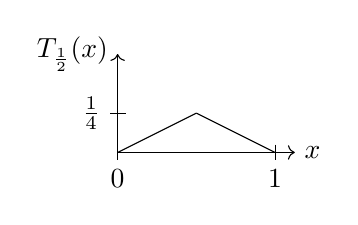
\begin{tikzpicture}[scale=2]
      \draw[->] (0.0,0.0) -- (1.125,0.0) node[right] {$x$};  
      \draw[->] (0.0,0.0) -- (0.0,0.625) node[left] {$T_{\frac{1}{2}}(x)$};
      \draw (0.0,0.0) -- (0.5,0.25);  
      \draw (0.5,0.25) -- (1.0,0.0);
      \draw (0,0.05) -- (0,-0.05) node[below] {$0$};
      \draw (1,0.05) -- (1,-0.05) node[below] {$1$};
      \draw (0.05,0.25) -- (-0.05,0.25) node[left] {$\frac{1}{4}$};
\end{tikzpicture}
\begin{tikzpicture}[scale=2]
      \draw[->] (0.0,0.0) -- (1.125,0.0) node[right] {$x$};  
      \draw[->] (0.0,0.0) -- (0.0,1.125) node[left] {$T_{\frac{3}{2}}(x)$};
      \draw (0.0,0.0) -- (0.5,0.75);  
      \draw (0.5,0.75) -- (1.0,0.0);
      \draw (0,0.05) -- (0,-0.05) node[below] {$0$};
      \draw (1,0.05) -- (1,-0.05) node[below] {$1$};
      \draw (0.05,0.75) -- (-0.05,0.75) node[left] {$\frac{3}{4}$};
\end{tikzpicture}
\begin{tikzpicture}[scale=2]
      \draw[->] (0.0,0.0) -- (1.125,0.0) node[right] {$x$};  
      \draw[->] (0.0,0.0) -- (0.0,1.875) node[left] {$T_{3}(x)$};
      \draw (0.0,0.0) -- (0.5,1.5);  
      \draw (0.5,1.5) -- (1.0,0.0);
      \draw (0,0.05) -- (0,-0.05) node[below] {$0$};
      \draw (1,0.05) -- (1,-0.05) node[below] {$1$};
      \draw (0.05,1.5) -- (-0.05,1.5) node[left] {$\frac{3}{2}$};
\end{tikzpicture}
\caption{Graf šotorske preslikave za različne $\mu$, omejene na $[0,1]$} \label{fig:M}  
\end{figure} 

\section{Dinamika preslikave za \texorpdfstring{$\mu \leq 2$}{m <= 2}}

Šotorska preslikava je definirana za vsa realna števila, vendar se je, kot bomo videli, smiselno omejiti na interval $[0,1]$.

\medskip

Naj bo $0 < \mu < 1$. Vemo že, da je $x=0$ fiksna točka. Če začnemo z $x \leq \frac{1}{2}$, iteriramo le še preslikavo $T_{\mu}(x) = \mu x$, saj je vrednost preslikave na vsakem koraku manjša od $\frac{1}{2}$, torej je $T_\mu^n(x) = \mu^n x$ za $x \in (-\infty, \frac{1}{2}]$. Če začnemo z $x \geq \frac{1}{2}$, za prvo iteracijo velja $T_\mu(x) < \frac{1}{2}$, zato po prvi iteraciji velja enako kot prej. Od tod sledi, da orbita poljubne točke $x \in \R$ konvergira k $0$.

\medskip

Pri $\mu = 1$ za $x \leq \frac{1}{2}$ velja $T_{\mu}(x) = x$, za $x \geq \frac{1}{2}$ pa $T_{\mu}(x) = 1 - x$. V takem sistemu so torej vse točke, ki so manjše ali enake $\frac{1}{2}$, fiksne, vse ostale točke pa so predperiodične fiksne točke.

\medskip

Za $\mu \in (1, 2)$ je obnašanje šotorske preslikave zanimivejše. Da dobimo boljšo predstavo o dogajanju v odvisnosti od $\mu$, lahko grafično prikažemo asimptotično obnašanje iteracije neke začetne točke, kot kaže slika \ref{pic:tent-bifurcation}.
\begin{figure}[h!]
\begin{center}
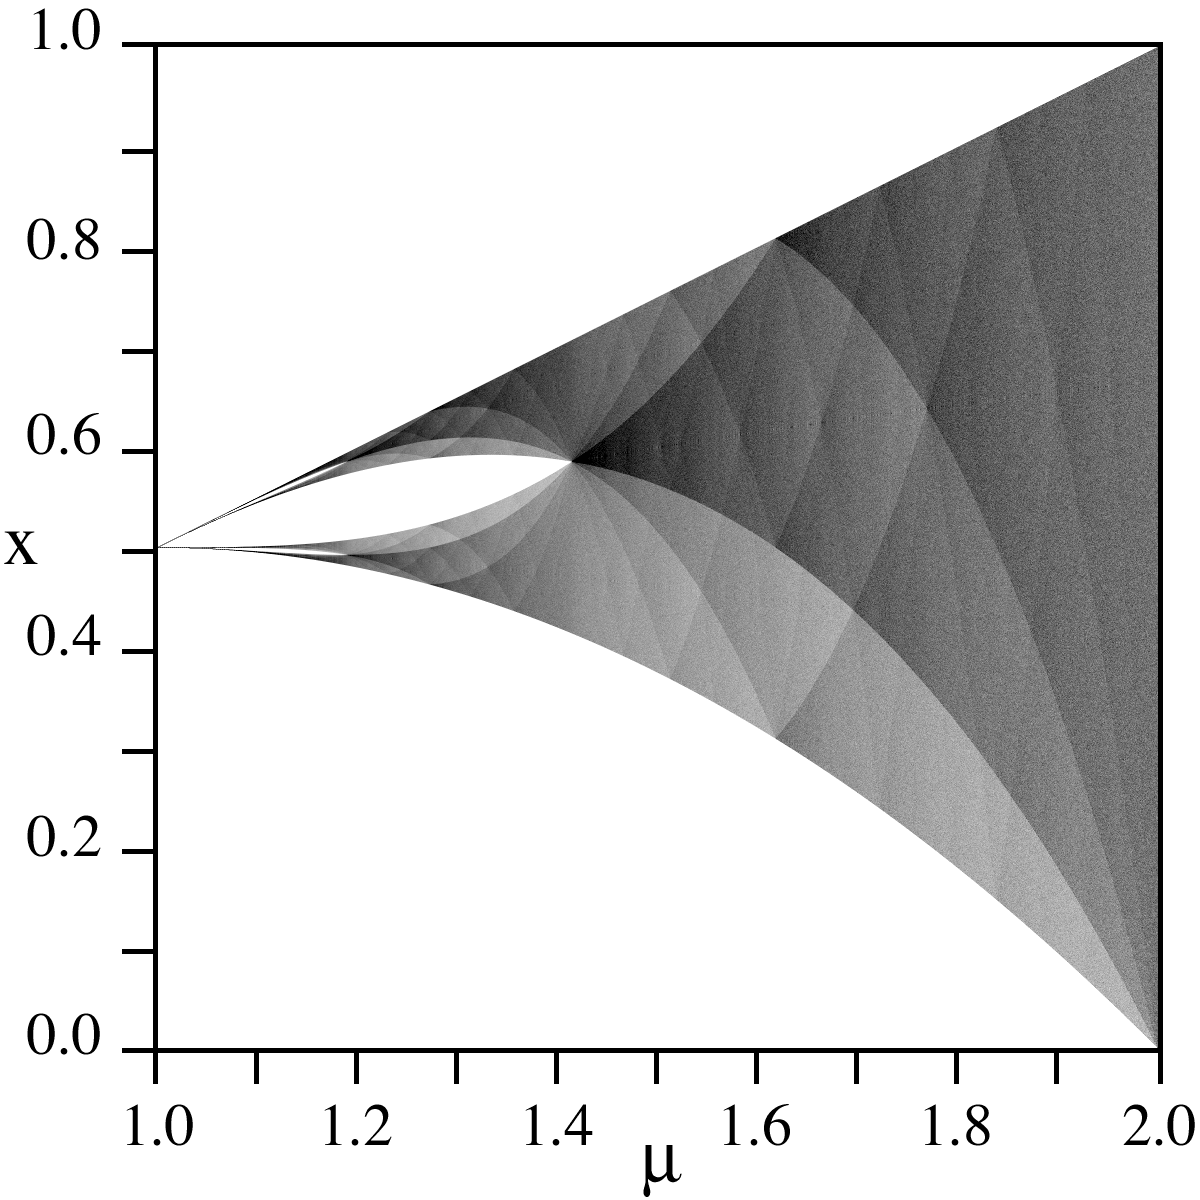
\includegraphics[width=0.65\textwidth]{img/tent_bifurcation.png}
\end{center}
\caption{Bifurkacijski diagram šotorske preslikave, vir: \cite{tentbif}}
\label{pic:tent-bifurcation}
\end{figure}

Dobljenemu diagramu pravimo \emph{bifurkacijski diagram}. Diagram na sliki \ref{pic:tent-bifurcation} prikazuje asimptotsko vedenje orbite $\gamma_{+}(\frac{1}{4})$. Opazimo, da vsi elementi orbite za vse $\mu \in (1,2)$ ostanejo na intervalu $[0,1]$. Kot navaja Ott v članku \cite{ott}, se izkaže, da orbita poljubne točke z intervala $(0,1)$ za $\mu \in (1,2]$ sčasoma postane ujeta na intervalu $(\mu - \frac{\mu^2}{2}, \frac{\mu}{2})$, kar vidimo tudi na bifurkacijskem diagramu \ref{pic:tent-bifurcation}. Izkaže se, da so orbite točk nestabilne, v smislu da se orbiti bližnjih začetnih točk razlikujeta (bližnje točke ne ostanejo blizu). Samo omenimo, da se tudi v tem primeru pojavi kaos.

Razmislimo, kaj se zgodi, če iteracijo začnemo s točko $x_0 \notin [0,1]$. Če je $x_0 \in (-\infty, 0)$, dobimo zaporedje $x_0, \mu x_0, \mu^2 x_0, \dots$, kjer $\mu^n$ raste neomejeno. Podobno velja za $x_0 \in (1, \infty)$, saj je $x_1 = \mu(1-x_0) < 0$. Zaporedje torej za $x_0 \notin [0,1]$ divergira proti $-\infty$. 

Smiselno je torej, da domeno omejimo na interval $[0,1]$. Potem lahko kodomeno prav tako omejimo na interval $[0,1]$, saj je preslikava $T_{\mu}$ na intervalu $[0,1]$ nenegativna in doseže maksimum v $T_\mu(\frac{1}{2}) = \frac{\mu}{2}$.

\medskip

Naj bo sedaj $\mu = 2$. Šotorska preslikava $T_2$ slika z intervala $[0, 1]$ nazaj na ta interval in je surjekcija. Namreč, za $y \in [0,1]$ vedno obstaja $x \leq \frac{1}{2}$, tako da je $T_2(x) = 2x = y$. Za občutek si na sliki \ref{pic:tent-2} poglejmo prve štiri iteracije $T_2$ na intervalu $[0,1]$. Vidimo, da $T_2$ sestoji iz dveh linearnih kosov, $T_2^2$ iz štirih linearnih kosov, $T_2^3$ iz osmih linearnih kosov in tako naprej. Vsak kos je definiran na $\frac{1}{2^n}$ deleža intervala $[0,1]$.

\begin{figure}[h!]
\begin{center}
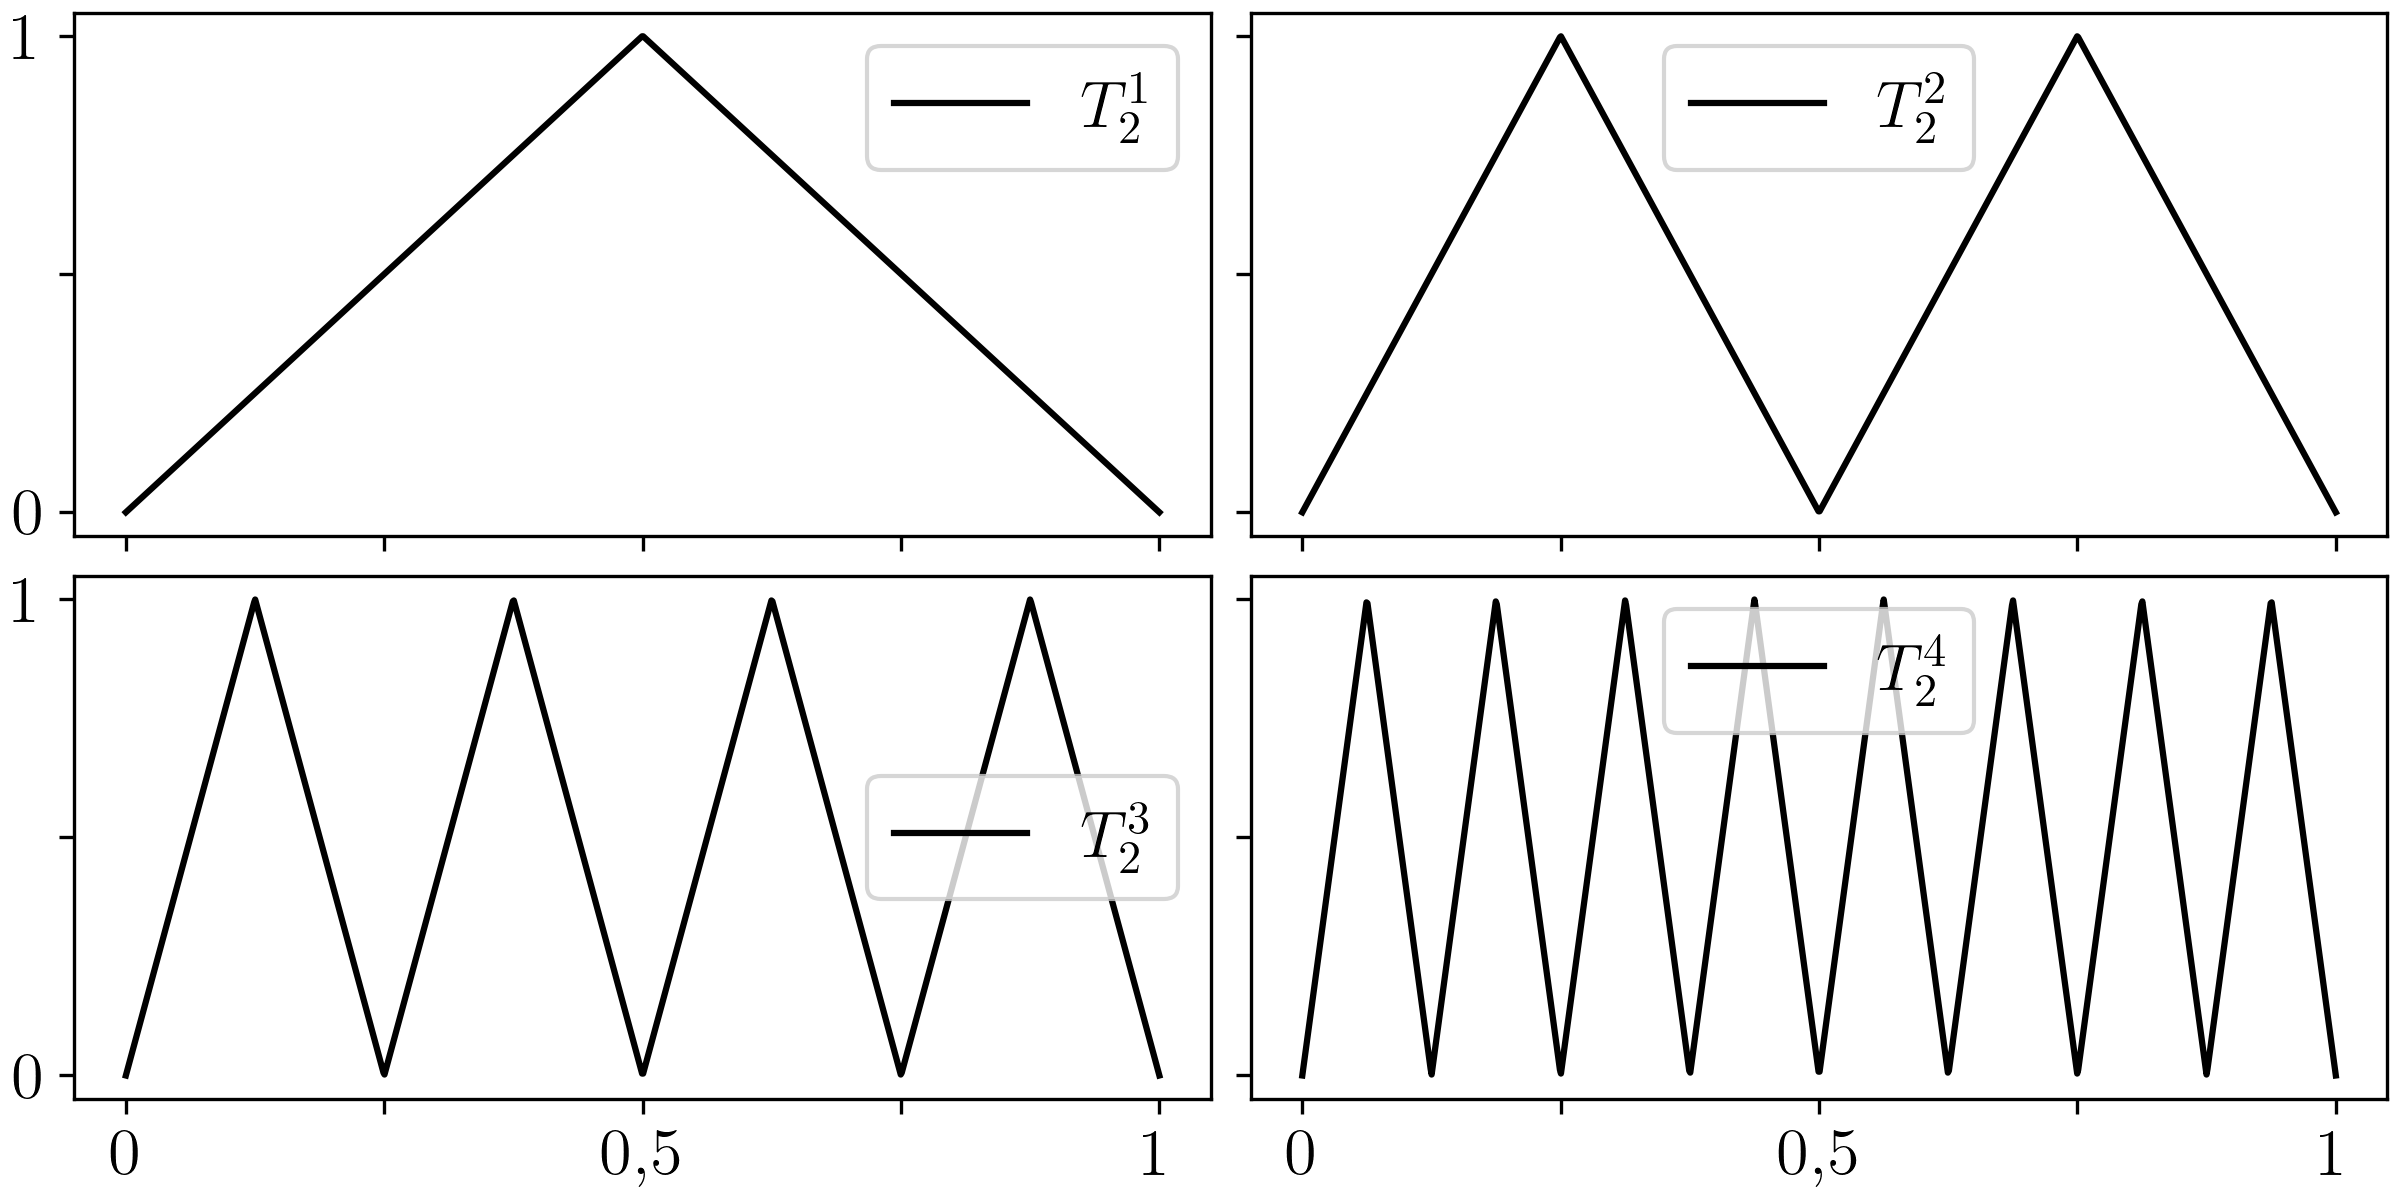
\includegraphics[width=0.9\textwidth]{img/tent_2.png}
\end{center}
\caption{Iteracije preslikave $T_2$}
\label{pic:tent-2}
\end{figure}

Tako je recimo
\begin{equation*}
T_2^2(x) =
\begin{cases}
4x\phantom{-2} \quad x \in [0, \frac{1}{4}] \\
2-4x \quad x \in [\frac{1}{4}, \frac{1}{2}] \\
4x-2 \quad x \in [\frac{1}{2}, \frac{3}{4}] \\
4x-4 \quad x \in [\frac{3}{4}, 1]
\end{cases}.
\end{equation*}
Ugotovitve strnemo v naslednji trditvi.

\begin{trditev}
Preslikava $T_2^n : [\frac{k}{2^n}, \frac{k+1}{2^n}] \rightarrow [0,1]$ je linearna in bijektivna za vse $0 \leq k \leq 2^n - 1$. 
\end{trditev}

\begin{dokaz}
Dokažimo z indukcijo na $n$. Za $n=1$ imamo dve zožitvi, $T_2: [0, \frac{1}{2}] \rightarrow [0,1]$ in $T_2: [\frac{1}{2}, 1] \rightarrow [0,1]$. Ker so za prvo zožitev vsi $x \in [0, \frac{1}{2}]$, je njen predpis $2x$, torej je $T_2: [0, \frac{1}{2}] \rightarrow [0,1]$ res linearna bijekcija. Za drugo zožitev je predpis $2 - 2x$, kar je spet linearna bijekcija.

\medskip

Naj je preslikava $T_2^n: [\frac{k}{2^n}, \frac{k+1}{2^n}] \rightarrow [0,1]$ linearna bijekcija za vse $0 \leq k \leq 2^n - 1$. Vzemimo interval $I = [\frac{k}{2^n}, \frac{k+1}{2^n}]$ za poljuben $k$. Dolžina tega intervala je $\frac{1}{2^n}$. Po predpostavki je $T_2^n: I \rightarrow [0,1]$ linearna in bijektivna. Kaj lahko povemo o preslikavi $T_2^{n+1}$?

Predpostavimo, da je $T_2^n: [a,b] \rightarrow [0,1]$ strogo naraščajoča. Potem je $T_2^n(\frac{k}{2^n}) = 0$ in $T_2^n(\frac{k+1}{2^n}) = 1$. Interval po sredini razdelimo na dva intervala, $I_1 = [\frac{2k}{2^{n+1}}, \frac{2k+1}{2^{n+1}}]$ in $I_2 = [\frac{2k+1}{2^{n+1}}, \frac{2k+2}{2^{n+1}}]$. Po linearnosti je $T_2^n(I_1) = [0, \frac{1}{2}]$, zato je $T_2^{n+1}: I_1 \rightarrow [0,1]$ linearna in bijektivna. Podobno velja $T_2^n(I_2) = [\frac{1}{2}, 1]$, zato je $T_2^{n+1}: I_2 \rightarrow [0,1]$ linearna in bijektivna. Če je $T_2^n$ padajoča, ravnamo podobno.

\medskip

Interval $I_1$ ustreza intervalu $[\frac{k'}{2^{n+1}}, \frac{k'+1}{2^{n+1}}]$ za $k' = 2k$, interval $I_2$ pa za $k' = 2k+1$. Ker je bil $k$ poljuben med $0$ in vključno $2^n-1$, tečejo $k'$ od $0$ do vključno $2 \cdot (2^n-1) + 1 = 2^{n+1} - 1$. S tem je trditev dokazana. \qedhere
\end{dokaz}

\bigskip

\begin{trditev}
Diskretni dinamični sistem $(M, T_2)$ za interval $M = [0,1]$ in preslikavo $T_2: M \rightarrow M$ je kaotičen.
\end{trditev}

\begin{dokaz}
Pokažimo najprej, da so periodične točke goste v $M$. Ker $T_2^n$ bijektivno preslika interval $[\frac{k}{2^n}, \frac{k+1}{2^n}]$ na interval $[0,1]$, ima $T_2^n(x) = x$ natanko eno rešitev in je $x$ periodična točka s periodo $n$. Ker lahko z večanjem $n$ pridemo z $x$ poljubno blizu vsaki točki iz $[0,1]$, so periodične točke goste v $[0,1]$.

Naj bosta $U$ in $V$ odprta podintervala od $[0,1]$. Za dovolj velik $n$ in za nek $0 \leq k \leq 2^n - 1$ množica $U$ vsebuje interval oblike $[\frac{k}{2^n}, \frac{k+1}{2^n}]$, torej je $T_2^n(U) = [0,1] \supset V$, zato je $T_2$ topološko tranzitivna.

Občutljivost na začetne pogoje sledi že po izreku \ref{izrek:obcutljivost}, vendar jo vseeno pokažimo. Naj bo $x \in [0,1]$ in izberimo poljuben $\varepsilon > 0$. Potem $\varepsilon$-okolica točke $x$ za dovolj velik $n$ vsebuje nek interval $I = [\frac{k}{2^n}, \frac{k+1}{2^n}]$. Za vsak $y \in I$ velja $d(x,y) < \varepsilon$. Ker je $T^n: I \rightarrow [0,1]$ bijekcija, obstaja tak $y \in I$, da je $d(T_2^n(x), T_2^n(y)) > \frac{1}{3} =: \delta$. \qedhere
\end{dokaz}

\section{Logistična preslikava}

Logistična preslikava je preslikava iz družine $h_r(x) = r x (1-x)$, kjer $r > 0$, in je sprejemljiv model rasti populacije. Za $r \leq 4$ velja, da $h$ slika z intervala $[0,1]$ nazaj na ta interval. Analiza obnašanja logistične preslikave v splošnem za razne $r \leq 4$ je zunaj okvira tega dela; na sliki \ref{fig:logistic-plot} je za občutek prikazana iteracija $h$ za nekaj različnih parametrov $r$ in začetno točko $x_0 = 0{,}35$. 

\begin{figure}[h!]
\begin{center}
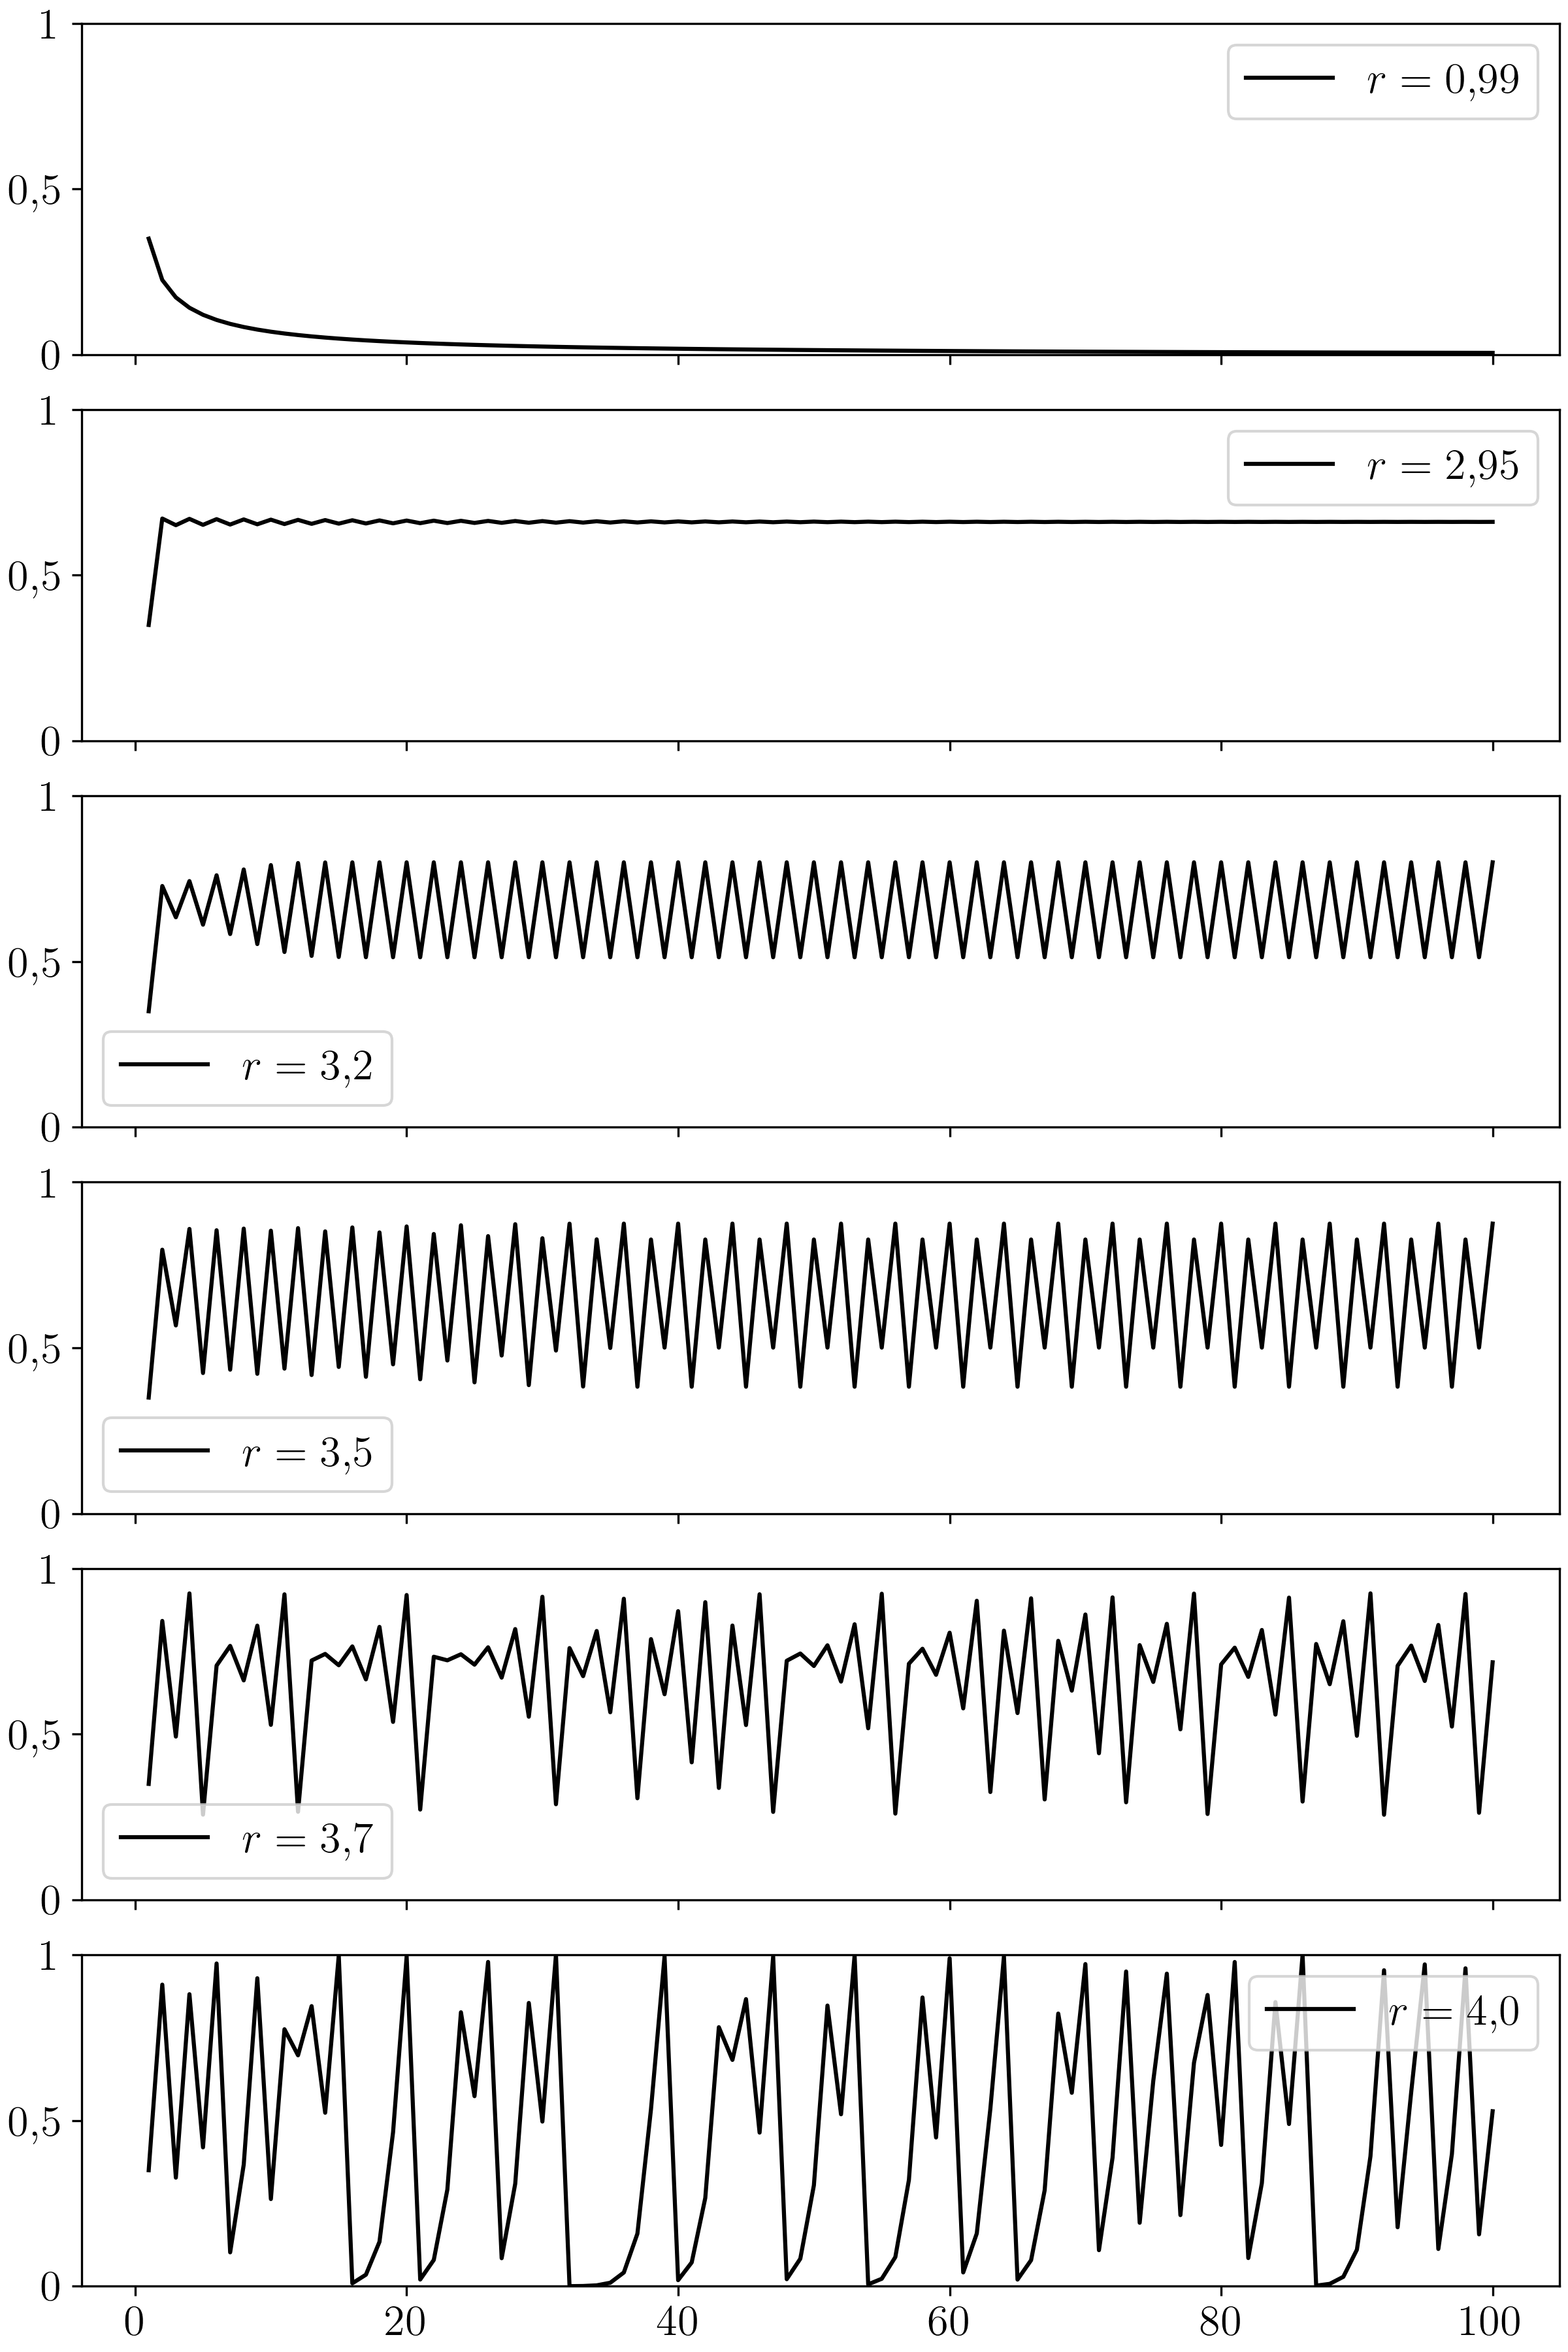
\includegraphics[width=0.6125\textwidth]{img/logistic_iteration.png}
\end{center}
\caption{Iteracija logistične preslikave za razne parametre $r$}
\label{fig:logistic-plot}
\end{figure}

\medskip

Povzemimo obnašanje, ki ga opisuje Holmgren v \cite{holmgren96}. Preslikava $h_r$ ima dve fiksni točki, to sta $0$ in $\frac{r-1}{r}$. Za $r < 1$ je privlačna fiksna točka $0$, za $r$ med $1$ in $3$ pa je privlačna fiksna točka $\frac{r-1}{r}$. Ko je $r$ med $3$ in $1+\sqrt{6}$, se pojavi cikel dolžine $2$. Ko je $r = 1+\sqrt{6}$, cikel dolžine $2$ preide v cikel dolžine $4$. Ko $r$ raste vse do $4$, se dinamika preslikave hitro spreminja.

\medskip

Dokaj enostavno lahko pokažemo, da je logistična preslikava kaotična za $r = 4$. Preden lahko to storimo, moramo pokazati, da topološka konjugacija ohranja kaotičnost sistema.

\begin{trditev}
\label{trditev:konjugacija-ohranjanje}
Naj bosta $X$ in $Y$ topološka prostora, naj bosta $f: X \rightarrow X$ in $g: Y \rightarrow Y$ preslikavi in naj bo $\varphi: X \rightarrow Y$ topološka konjugacija $f$ in $g$. Potem velja:
\begin{itemize}
    \item inverz $\varphi^{-1}: Y \rightarrow X$ je topološka konjugacija,
    \item za vsak $n \in \N$ je $\varphi \circ f^n = g^n \circ \varphi$,
    \item periodične točke $f$ so goste v $X$, natanko tedaj ko so periodične točke $g$ goste v $Y$ in
    \item $f$ je topološko tranzitivna na $X$, natanko tedaj ko je $g$ topološko tranzitivna na $Y$.
\end{itemize}
\end{trditev}

\begin{dokaz}
Ker je $\varphi$ homeomorfizem, je očitno tudi inverz $\varphi^{-1}$ homeomorfizem. Pokazati moramo torej le, da je $\varphi^{-1} \circ g = f \circ \varphi^{-1}$. Ker je $\varphi$ topološka konjugacija, velja $\varphi \circ f = g \circ \varphi$. Potem je $\varphi^{-1} \circ \varphi \circ f = \varphi^{-1} \circ g \circ \varphi$, torej $f=\varphi^{-1} \circ g \circ \varphi$. Komponirajmo še z inverzom z desne in dobimo $f \circ \varphi^{-1} =\varphi^{-1} \circ g \circ \varphi \circ \varphi^{-1}$ oziroma ekvivalentno $f \circ \varphi^{-1} =\varphi^{-1} \circ g$, kar je ravno to, kar želimo pokazati.

\smallskip

Pokažimo, da za vsak $n \in \N$ velja $\varphi \circ f^n = g^n \circ \varphi$. Enakost velja za $n=1$, saj je $\varphi$ topološka konjugacija. Predpostavimo, da velja $\varphi \circ f^n = g^n \circ \varphi$. Potem velja tudi $\varphi \circ f^{n+1} = g^{n+1} \circ \varphi$, saj je $\varphi \circ f^{n+1} = (\varphi \circ f^n) \circ f = (g^n \circ \varphi) \circ f = g^n \circ (\varphi \circ f) = g^n \circ (g \circ \varphi) = g^{n+1} \circ \varphi.$

\smallskip

Naj so periodične točke $f$ goste v $X$. Vzemimo poljubno odprto množico $V$ iz $Y$. Ker je $\varphi$ homeomorfizem, je zvezna, zato je praslika $U=f^{-1}(V)$ odprta množica v $X$. Ker so periodične točke goste v $X$, množica $U$ vsebuje periodične točke $f$. Izberimo poljubno periodično točko $p \in U$ in njeno periodo označimo z $n$, torej $f^n(p) = p$. Potem je to tudi periodična točka v množici $V$, saj je $\varphi(f^n(p)) = g^n(\varphi(p))$. Ker poljubna odprta množica $V$ iz $Y$ vsebuje periodično točko, so periodične točke goste v $Y$. Ker je tudi $\varphi^{-1}$ topološka konjugacija, velja implikacija tudi v drugo smer.

\smallskip

Naj bo $f$ topološko tranzitivna na $X$. Vzemimo poljubni odprti množici $U_Y$ in $V_Y$ v $Y$. Ker je $\varphi$ homeomorfizem, je zvezna, torej sta prasliki $U_X = \varphi^{-1}(U_Y)$ in $V_X = \varphi^{-1}(V_Y)$ odprti množici. Ker je $f$ topološko tranzitivna, obstaja tak $n \in \N$, da je presek $f^n(U_X) \cap V_X$ neprazen. Ker je $\varphi$ homeomorfizem, je tudi množica $\varphi(f^n(U_X) \cap V_X)$ neprazna. Če uporabimo topološko konjugacijo, dobimo
\begin{align*}
    \emptyset &\neq \varphi(f^n(U_X) \cap V_X) \\
    &\subseteq \varphi(f^n(U_X)) \cap \varphi(V_X) \\
    &= g^n(\varphi(U_X)) \cap \varphi(V_X) \\
    &= g^n(U_Y) \cap V_Y,
\end{align*}
zato je $g$ topološko tranzitivna na $Y$. Ker je tudi $\varphi^{-1}$ topološka konjugacija, velja implikacija tudi v drugo smer. \qedhere
\end{dokaz}

\medskip

\begin{trditev}
Preslikava $h: [0,1] \rightarrow [0,1], \; h(x) = 4x(1-x)$ je kaotična.
\end{trditev}

\begin{dokaz}
Pokazali smo že, da je šotorska preslikava $T_2: [0,1] \rightarrow [0,1]$ kaotična. Vzemimo preslikavo $\varphi: [0,1] \rightarrow [0,1], \; \varphi(x) = \sin^2(\frac{\pi}{2}x)$ in preverimo, da je $\varphi$ topološka konjugacija med $T_2$ in $h$.

Dokažimo, da je $\varphi$ injektivna. Vzemimo sliki $y_1 = y_2$ funkcije $\varphi$. Ker je $y_1 = y_2 \iff \sin^2(\frac{\pi}{2}x_1) = \sin^2(\frac{\pi}{2}x_2) \iff \sin(\frac{\pi}{2}x_1) = \sin(\frac{\pi}{2}x_2) \iff x_1 = x_2$, je $\varphi$ res injekcija. Naj bo $y \in [0,1]$. $\varphi$ je surjekcija:
\begin{align*}
    &\sin^2(\frac{\pi}{2} x) = y \\
    \llap{$\iff$ \quad} &\sin(\frac{\pi}{2} x) = \sqrt{y} \quad (\text{koren bijekcija na } [0,1]) \\
    \llap{$\iff$ \quad} &\frac{\pi}{2} x = \arcsin(\sqrt{y}) \quad (\arcsin \text{ bijekcija na } [0,1]) \\
    \llap{$\iff$ \quad} &x = \underbrace{\frac{2}{\pi} \arcsin(\sqrt{y})}_{\in [0,1] \text{ za } y \in [0,1]}
\end{align*}

Sledi, da je $\varphi$ bijekcija na $[0,1]$, z inverzom $\varphi^{-1}(x) = \frac{2}{\pi} \arcsin(\sqrt{x})$. Ker je kompozitum zveznih preslikav prav tako zvezna preslikava, sta tako $\varphi$ kot inverz $\varphi^{-1}$ zvezna.

Po eni strani velja
\begin{align*}
    (\varphi \circ T_2)(x) &= \varphi(2 \min(x, 1-x)) \\
    &= 
    \begin{cases} 
    \sin^2(\pi x) &\quad \text{za } x \leq\frac{1}{2} \\
    \sin^2(\pi - \pi x) &\quad \text{za } x \geq \frac{1}{2}
    \end{cases} \\
    &= \sin^2(\pi x),
    \intertext{in po drugi strani velja}
    (h \circ \varphi)(x) &= h(\sin^2(\frac{\pi}{2} x) \\
    &= 4 \sin^2(\frac{\pi}{2} x) (1 - \sin^2(\frac{\pi}{2} x)) \\
    &= 4 \sin^2(\frac{\pi}{2} x) \cos^2(\frac{\pi}{2} x) \\
    &= (2 \sin(\frac{\pi}{2} x) \cos(\frac{\pi}{2} x))^2 \\
    &= \sin^2(\pi x),
\end{align*}
zato je $\varphi$ res topološka konjugacija. Potem po trditvi \ref{trditev:konjugacija-ohranjanje} velja, da so periodične točke preslikave $h$ goste v $[0,1]$ in da je $h$ topološko tranzitivna. Ker je $h$ zvezna, je $h$ po izreku \ref{izrek:obcutljivost} občutljiva na začetne pogoje, torej je kaotična.  \qedhere
\end{dokaz}

\section{Cantorjeve množice}

Šotorska preslikava $T_\mu$ za vrednosti parametra $\mu > 2$ z intervala $[0,1]$ ne slika več na ta interval, ampak na večji interval $[0, \frac{\mu}{2}]$. Pri dveh iteracijah dobimo
\begin{align*}
    &T_\mu : [0,1] \longrightarrow [0, \frac{\mu}{2}] \quad \text{in} \\
    &T^2_\mu : [0, 1] \longrightarrow [\mu - \frac{\mu^2}{2}, \frac{\mu}{2}].
\end{align*}

Ker imamo po drugi iteraciji slike, ki so negativne, se v nadaljnjih iteracijah interval še bolj širi proti $-\infty$. Dinamični sistem bi torej lahko obravnavali na množici $(-\infty, \frac{\mu}{2}]$, vendar je dogajanje na negativni strani tega intervala \narekovaji{nezanimivo}, saj se razdalja med iterati na vsakem koraku poveča za faktor $\mu$ in zaporedje divergira proti $-\infty$. 

Raje omejimo prostor, na katerem je definirana $T_\mu$, na le tista števila, ki pri iteraciji ostanejo na intervalu $[0,1]$. Za vsako naravno število $n$ definirajmo množico
\begin{equation*}
    \Lambda_n = \set{ x \in [0,1] \mid T_\mu^n(x) \in [0,1] }.
\end{equation*}

\medskip

Za parametre $\mu > 2$ velja, da je $T_\mu^n(x) \in [0,1]$ ekvivalentno temu, da je $T_\mu^k(x) \in [0,1]$ za vsak $0 \leq k \leq n$. Potem je množica $$ \Lambda = \bigcap_{n \in \N} \Lambda_n $$ množica točk, ki pri iteraciji za vedno ostanejo na intervalu $[0,1]$. Po konstrukciji je množica $\Lambda$ invariantna, to je $T_\mu(\Lambda) = \Lambda$. Obravnavamo lahko torej dinamični sistem $(\Lambda, T_\mu)$. Najprej razmislimo, kakšna je množica $\Lambda$. Za lažjo predstavo si na sliki \ref{fig:tent_iter_3} oglejmo prve štiri iteracije preslikave $T_3$. Vidimo, da $T_3$ slika dva disjunktna intervala na $[0,1]$, $T_3^2$ slika po dva intervala iz obeh prejšnjih intervalov na $[0,1]$, in tako naprej.

\begin{figure}[h!]
\begin{center}
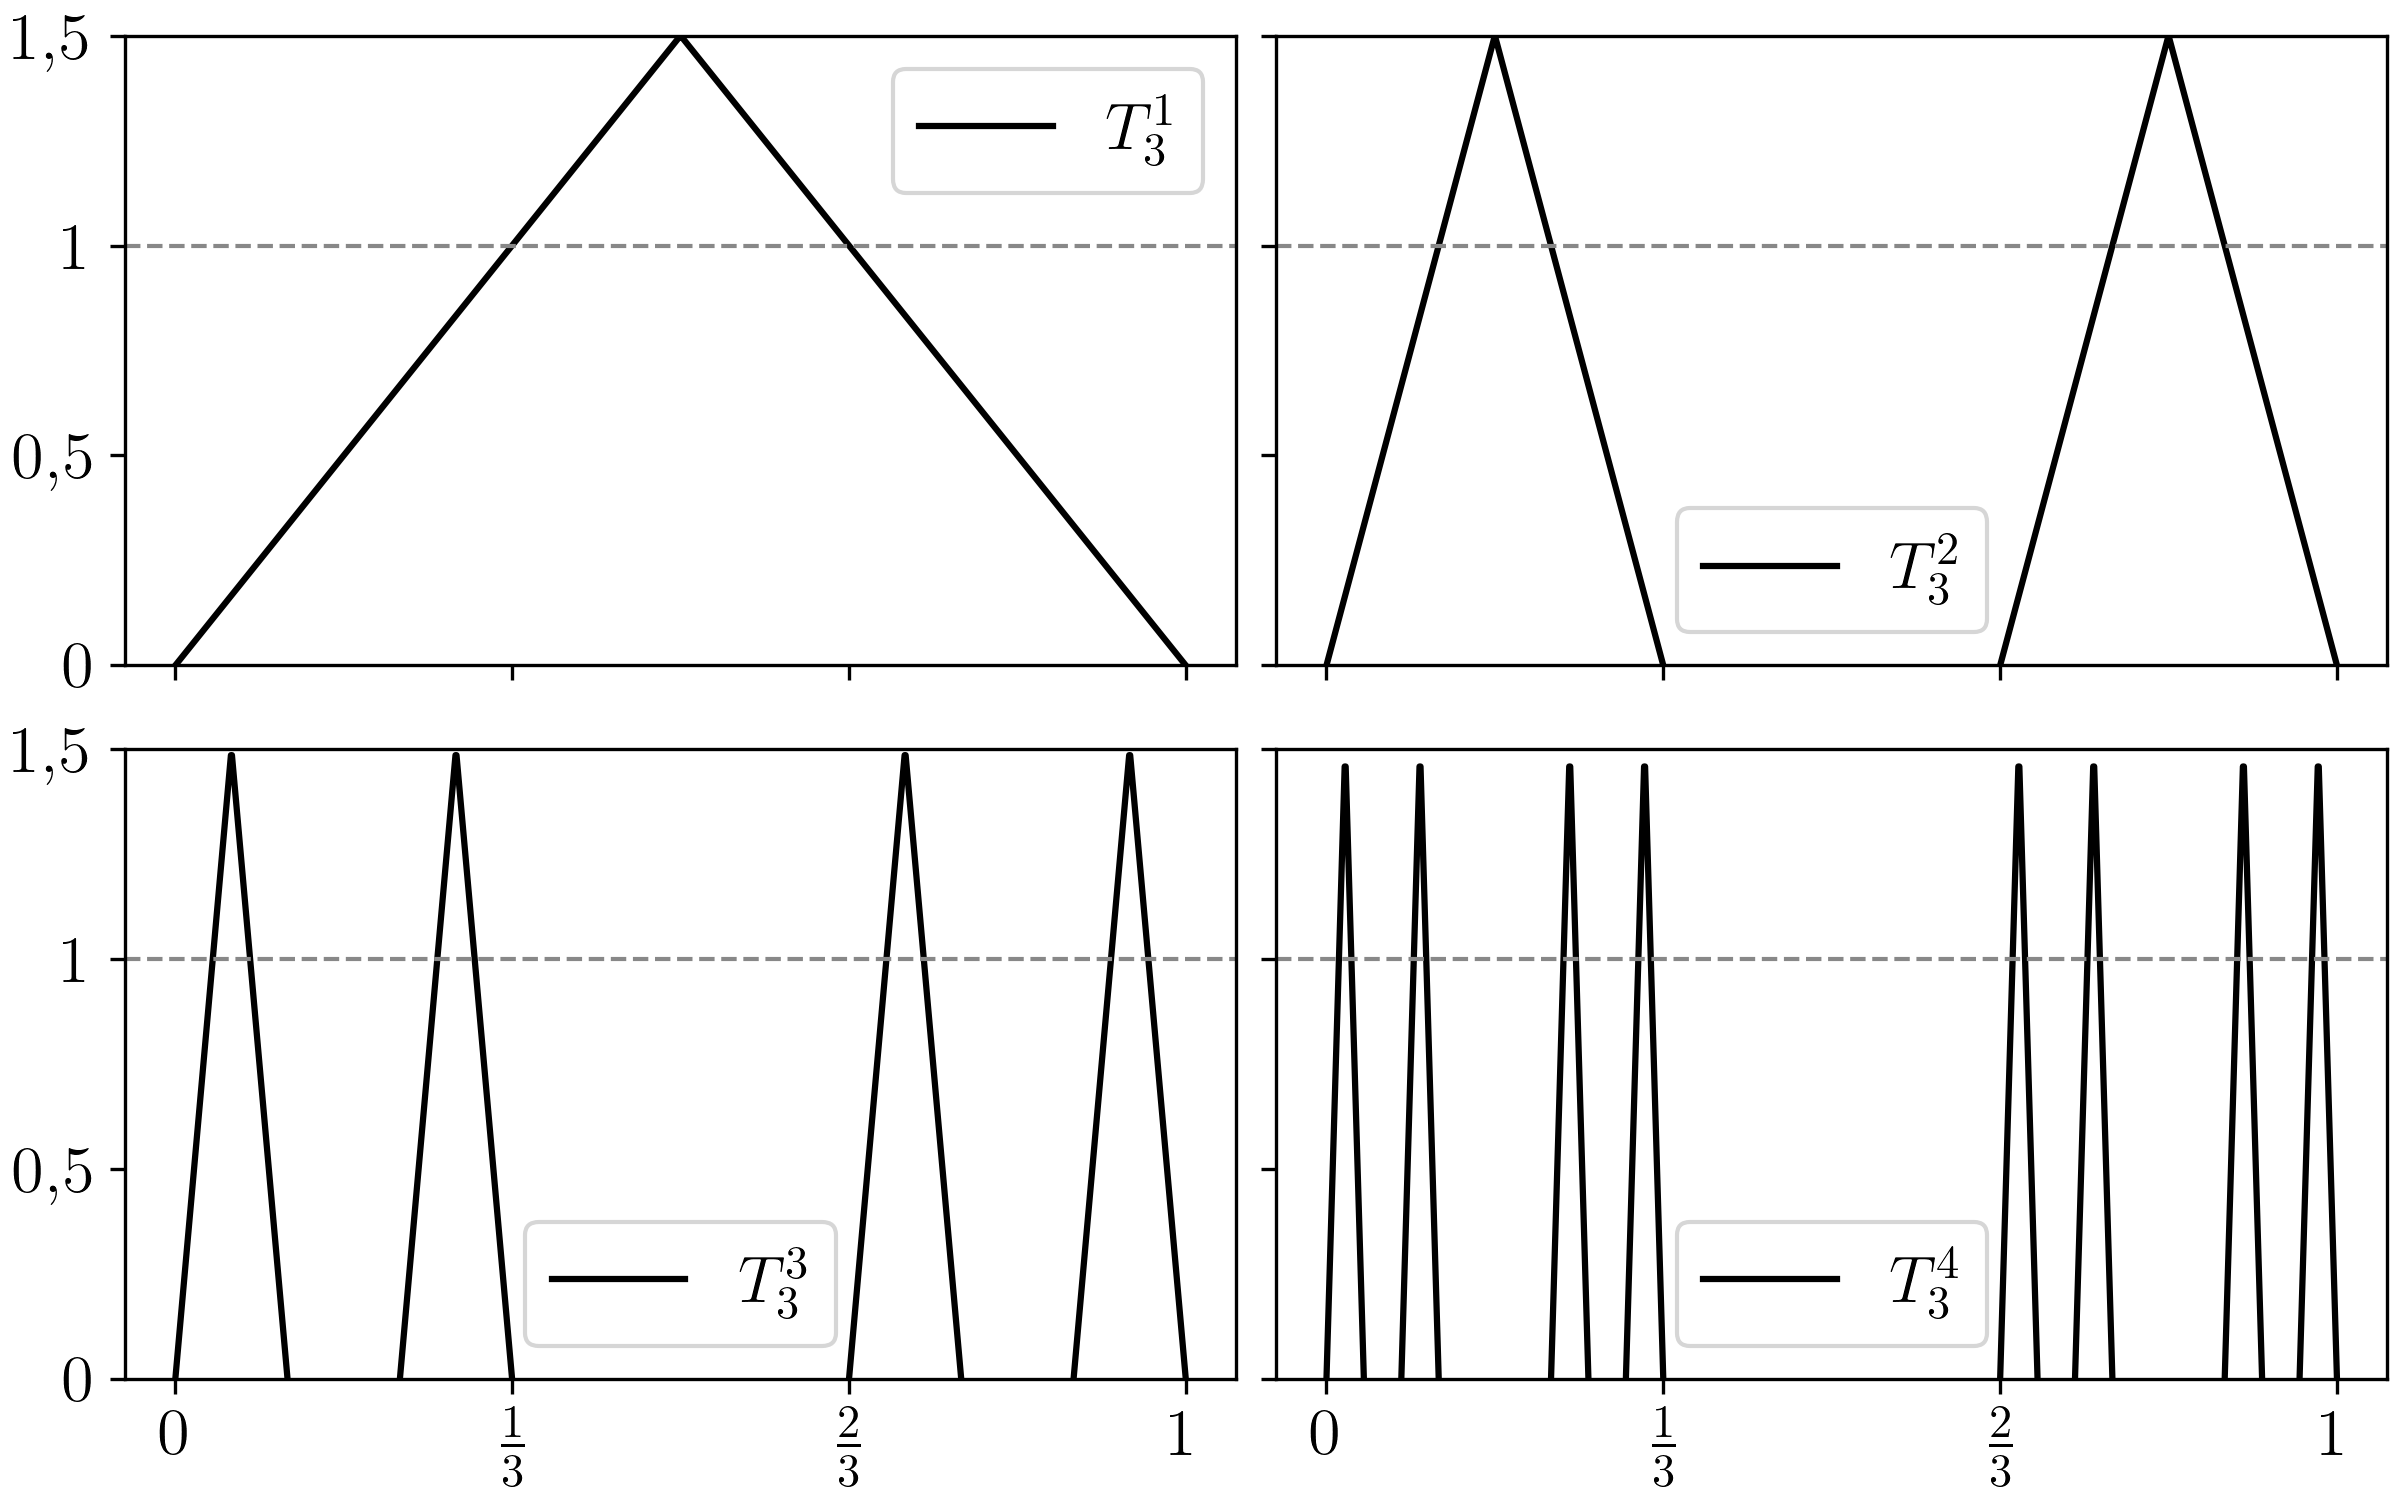
\includegraphics[width=0.9\textwidth]{img/tent_3.png}
\end{center}
\caption{Iteracija preslikave $T_3$}
\label{fig:tent_iter_3}
\end{figure}

\begin{trditev}
\label{trditev:lambda_1}
Množica točk, ki po prvi iteraciji $T_\mu$ ostane na intervalu $[0,1]$, je $\Lambda_1 = [0, \frac{1}{\mu}] \cup [1-\frac{1}{\mu}, 1]$.
\end{trditev}

\begin{dokaz}
Ločimo dva primera. Za $x \in [0, \frac{1}{2}]$ je $T_\mu(x) = \mu x$, in ker želimo $T_\mu(x) \leq 1$, mora biti $x \leq \frac{1}{\mu} < \frac{1}{2}$. Po drugi strani, za $x \in [\frac{1}{2}, 1]$, je $T_\mu(x) = \mu (1-x)$, od koder dobimo $x \geq \frac{\mu - 1}{\mu} = 1 - \frac{1}{\mu}$. 

Torej je res $\Lambda_1 = [0, \frac{1}{\mu}] \cup [1-\frac{1}{\mu}, 1]$. \qedhere
\end{dokaz}

\bigskip

\begin{trditev}
\label{trditev:lambda_zgradba}
Množica $\Lambda_n$ je unija $2^n$ disjunktnih zaprtih intervalov. Če je $I = [a,b]$ eden od teh intervalov, je njegova dolžina $(\frac{1}{\mu})^n$ in preslikava $T_\mu^n: I \rightarrow [0,1]$ je linearna.
\end{trditev}

\begin{dokaz}
Trditev dokažimo z indukcijo. Po trditvi \ref{trditev:lambda_1} je $\Lambda_1$ unija dveh disjunktnih zaprtih intervalov $I_0 = [0, \frac{1}{\mu}]$ in $I_1 = [1-\frac{1}{\mu}, 1]$. Dolžina obeh intervalov je $\frac{1}{\mu}$. Preverimo, da sta obe zožitvi linearni.
\begin{itemize}
    \item Za $T_\mu: I_0 \rightarrow [0,1]$ velja $T_\mu(x) = \mu x$, saj je $x < \frac{1}{2}$ za vse $x \in I_0$. Preslikava je očitno linearna.
    \item Za $T_\mu: I_1 \rightarrow [0,1]$ velja $T_\mu(x) = \mu (1-x)$, saj je $x > \frac{1}{2}$ za vse $x \in I_0$. Podobno kot prej je preslikava linearna.
\end{itemize}
S tem je dokazana baza indukcije.

\bigskip

Predpostavimo sedaj, da je množica $\Lambda_n$ unija $2^n$ disjunktnih in zaprtih intervalov in da je preslikava $T_\mu^n: I \rightarrow [0,1]$ linearna za vsak $I \in \Lambda_n$. Fiksirajmo poljuben interval $I = [a,b] \in \Lambda_n$, ki ima po indukcijski predpostavki dolžino $(\frac{1}{\mu})^n$. Oglejmo si, kaj lahko povemo o množici $\Lambda_{n+1}$ oziroma bolj specifično, katere točke iz intervala $I \in \Lambda_n$ so tudi v $\Lambda_{n+1}$. Ločimo dva primera, glede na to, ali je $T_\mu^n$ strogo naraščajoča ali strogo padajoča.

\medskip

Privzemimo najprej, da je $T_\mu^n$ strogo naraščajoča linearna preslikava z intervala $I$ na $[0,1]$. Potem je njen predpis $T_\mu^n(x) = \mu^n (x-a)$. Naj bosta $c = a + \frac{1}{\mu^{n+1}}$ in $d = b - \frac{1}{\mu^{n+1}}$. Ker je $T_\mu^n(c) = \frac{1}{\mu}$ in ker je $T_\mu^n(d) = 1 - \frac{1}{\mu}$, lahko preslikavi $T_\mu^n$ priredimo tri zožitve:
\begin{itemize}
    \item $T_\mu^n : [a, c] \rightarrow [0, \frac{1}{\mu}]$,
    \item $T_\mu^n : (c, d) \rightarrow (\frac{1}{\mu}, 1-\frac{1}{\mu})$ in
    \item $T_\mu^n : [d, b] \rightarrow [1-\frac{1}{\mu}, 1]$.
\end{itemize}
Če naredimo še eno iteracijo preslikave $T_\mu$, velja:
\begin{itemize}
    \item $T_\mu^{n+1}([a, c]) = [0,1]$,
    \item $T_\mu^{n+1}([d, b]) = [0,1]$ in
    \item $T_\mu^{n+1}(x) > 1$ za vse $x \in (c, d)$.
\end{itemize}
Množica točk z intervala $I = [a,b] \in \Lambda_n$, ki so tudi del $\Lambda_{n+1}$, je torej unija dveh disjunktnih zaprtih intervalov $[a, c]$ in $[d, b]$. Oba intervala imata dolžino $(a + \frac{1}{\mu^{n+1}}) - a = b - (b - \frac{1}{\mu^{n+1}}) = \frac{1}{\mu^{n+1}}$. Premislimo še, da sta preslikavi $T_\mu^{n+1} : [a, c] \rightarrow [0, 1]$ in $T_\mu^{n+1} : [d, b] \rightarrow [0, 1]$ linearni. Ker je $T_\mu^n : [a, c] \rightarrow [0, \frac{1}{\mu}]$ linearna po predpostavki, je tudi $T_\mu^{n+1} = \mu T_\mu^n$ linearna. Podobno velja za $T_\mu^{n+1} : [d, b] \rightarrow [0, 1]$.

\medskip

Podobno velja, če je $T_\mu^n: I \rightarrow [0,1]$ strogo padajoča linearna preslikava. Prav tako dobimo za $c = a + \frac{1}{\mu^{n+1}}$ in $d = b - \frac{1}{\mu^{n+1}}$ intervala $[a,c]$ in $[d,b]$, tako da je $T_\mu^{n+1}([a, c]) = [0,1]$ in $T_\mu^{n+1}([d, b]) = [0,1]$.

\medskip

Ker je $I = [a,b]$ poljuben interval iz $\Lambda_n$ in smo iz njega dobili dva intervala v $\Lambda_{n+1}$, ima $\Lambda_{n+1}$ dvakrat več intervalov kot $\Lambda_n$, torej $\Lambda_{n+1}$ vsebuje $2^{n+1}$ disjunktnih zaprtih intervalov. Pokazali smo tudi, da je preslikava $T_\mu^{n+1}: I \rightarrow [0,1]$ linearna za vsak interval $I \in \Lambda_{n+1}$. \qedhere
\end{dokaz}

\bigskip

Spomnimo se, da želimo opisati množico $\Lambda = \bigcap_{n \in \N} \Lambda_n$. Konstrukcija množic $\Lambda_n$ spominja na tipično konstrukcijo Cantorjeve množice.

\smallskip

\begin{definicija}
Neprazna množica $\Gamma \subset \R$ je \emph{Cantorjeva množica}, če velja:
\begin{enumerate}
    \item $\Gamma$ je zaprta in omejena,
    \item $\Gamma$ ne vsebuje intervalov in
    \item vsaka točka v $\Gamma$ je stekališče od $\Gamma$.
\end{enumerate}
\end{definicija}

Cantorjeve množice običajno zgradimo z iterativnimi postopki. Začnimo z intervalom $\cantorset_0 = [0, 1]$. Na vsakem koraku iz preostalih intervalov prejšnje iteracije odstranimo sredinsko tretjino. Tako v prvem koraku odstranimo odprt interval $(\frac{1}{3}, \frac{2}{3})$, da dobimo $\cantorset_1 = [0, \frac{1}{3}] \, \cup \, [\frac{2}{3}, 1]$. V drugem koraku odstranimo intervala $(\frac{1}{9}, \frac{2}{9})$ in $(\frac{7}{9}, \frac{8}{9})$, da dobimo $\cantorset_2 = [0, \frac{1}{9}] \, \cup \, [\frac{2}{9}, \frac{3}{9}] \, \cup \, [\frac{6}{9}, \frac{7}{9}] \, \cup \, [\frac{8}{9}, 1]$, in tako naprej. Postopek je prikazan na sliki \ref{fig:cantor_construction}.

\begin{figure}[h!]
\begin{center}
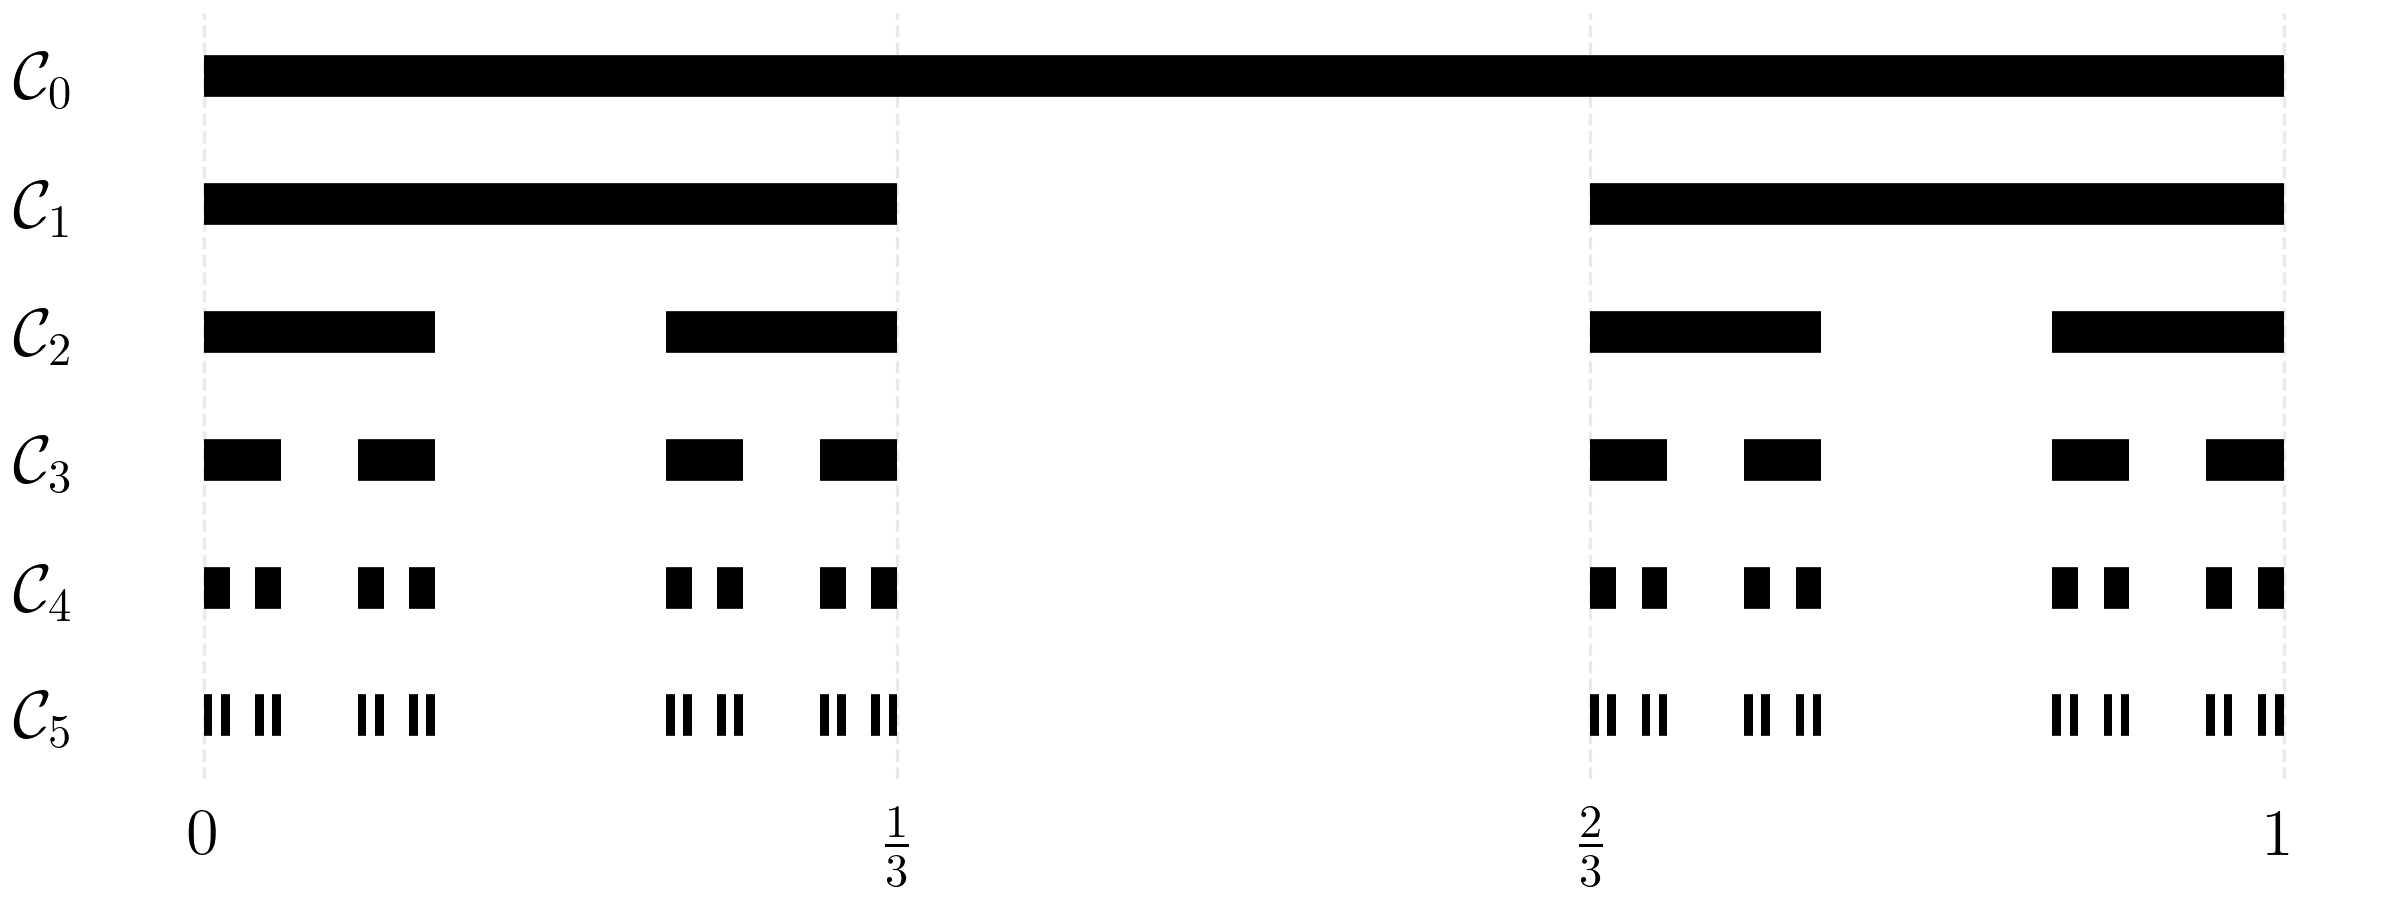
\includegraphics[width=0.9\textwidth]{img/cantor_set.png}
\end{center}
\caption{Iteracijska konstrukcija množic $\cantorset_n$}
\label{fig:cantor_construction}
\end{figure}

Pokažimo, da z zgoraj opisanim iterativnim postopkom dobimo Cantorjevo množico. Pri tem iterativni postopek posplošimo, tako da iz intervalov ne odstranjujemo sredinske tretjine, ampak poljuben sredinski delež, ki ga označimo z $\alpha$, tako da $0 < \alpha < 1$. Če iz poljubnega intervala odstranimo sredinski delež $\alpha$, na vsaki strani ostane delež $\beta := \frac{1-\alpha}{2}$. 

Zapišimo, kako izgledajo $\cantorset_0$, $\cantorset_1$ in $\cantorset_2$.
\begin{align*}
\cantorset_0 &= [0, 1] \\
\cantorset_1 &= [0, \beta] \cup [1 - \beta, 1] \\
\cantorset_2 &= [0, \beta^2] \cup [\beta - \beta^2, \beta] \cup [1 - \beta, 1 - \beta + \beta^2] \cup [1 - \beta^2, 1] \\
\vdots \phantom{.} &
\end{align*}

Pokažimo, kako je zgrajena množica $\cantorset_n$.

\begin{lema}
Množica $\cantorset_n$ vsebuje $2^n$ disjunktnih zaprtih intervalov, ki imajo skupno dolžino $(1-\alpha)^n$. Dolžina posameznega intervala je $(\frac{1-\alpha}{2})^n$.
\end{lema}

\begin{dokaz}
Lemo dokažimo z indukcijo. Množica $\cantorset_0$ ima res $2^0 = 1$ zaprt interval, ki ima dolžino $(\frac{1-\alpha}{2})^0 = 1$. 

Predpostavimo sedaj, da $\cantorset_n$ vsebuje $2^n$ disjunktnih intervalov in ima vsak dolžino $(\frac{1-\alpha}{2})^n$. Pri konstrukciji množice $\cantorset_{n+1}$ iz vsakega intervala $I$ iz $\cantorset_n$ dobimo dva intervala, ki sta vsebovana v $I$, zato ima nova množica $2 \cdot 2^n = 2^{n+1}$ disjunktnih intervalov. Iz vsakega intervala smo dobili dva nova intervala in odstranili delež $\alpha$, zato je dolžina vsakega novega intervala enaka $\frac{1}{2} \cdot (1-\alpha) \cdot (\frac{1-\alpha}{2})^n = (\frac{1-\alpha}{2})^{n+1}$.

Ker $\cantorset_n$ vsebuje $2^n$ zaprtih intervalov in ima vsak dolžino $(\frac{1-\alpha}{2})^n$, je njihova skupna dolžina $2^n \cdot (\frac{1-\alpha}{2})^n = (1-\alpha)^n$. \qedhere
\end{dokaz}

\begin{trditev}
Množica $$\cantorset = \bigcap_{n \in \N_0} \cantorset_n$$ je Cantorjeva množica.
\end{trditev}

\begin{dokaz}
Pokažimo, da množica $\cantorset$ izpolnjuje vse zahteve iz definicije. Množica $\cantorset$ je neprazna, saj vsaka $\cantorset_n$ vsebuje točki $0$ in $1$. 
\begin{enumerate}
    \item Množica $\cantorset$ je zaprta, saj je presek zaprtih intervalov, in omejena, saj je $\cantorset \subset \cantorset_0 = [0, 1]$.
    \item Recimo, da $\cantorset$ vsebuje interval $(a, b)$ z dolžino $d$. Potem mora biti $(a,b) \in \cantorset_n$ za vsak $n$. Ker ima množica $\cantorset_n$ po prejšnji lemi skupno dolžino intervalov $(1-\alpha)^n$, lahko najdemo tak $n_0$, da je $d < (1-\alpha)^{n_0}$. Ker je skupna dolžina vseh intervalov v $\cantorset_{n_0}$ manjša od $d$, množica $\cantorset_{n_0}$ ne more vsebovati intervala $(a,b)$. Predpostavka, da $\cantorset$ vsebuje interval, je vodila v protislovje, zato $\cantorset$ ne vsebuje intervalov.
    \item Naj bo $x \in \cantorset$ in naj bo $K_\varepsilon(x)$ odprta krogla s polmerom $\varepsilon$ okoli $x$. Pokazati moramo, da v $\cantorset$ obstaja točka $y$, tako da $x \neq y$ in $y \in K_\varepsilon(x)$. Ker je $x \in \cantorset$, za vsak $n$ obstaja interval v $\cantorset_n$, ki vsebuje $x$. Izberimo dovolj velik $n$, tako da $(\frac{1-\alpha}{2})^n < \varepsilon$ in z $I_n$ označimo interval, na katerem je $x$. Ker je dolžina tega intervala $(\frac{1-\alpha}{2})^n$, krogla $K_\varepsilon(x)$ vsebuje obe krajišči intervala $I_n$. Ker so krajišča intervalov iz $\cantorset_n$ v $\cantorset$, in eno od teh krajišč zagotovo ni enako $x$, smo našli točko $y \in \cantorset$, ki je v $K_\varepsilon(x)$. \qedhere
\end{enumerate}
\end{dokaz}

\medskip

\begin{trditev}
Množica $\Lambda = \bigcap_{n \in \N_0} \Lambda_n$ je Cantorjeva množica.
\end{trditev}

\begin{dokaz}
Spomnimo se, da je množica $\Lambda_n$ definirana kot
\begin{equation*}
\Lambda_{n} = \set{ x \in [0,1] \mid T_\mu^n(x) \in [0,1] }.
\end{equation*}

Za $n = 0$ velja $\Lambda_0 = [0,1]$. Po definiciji $\Lambda_n$ sledi, da je $\Lambda_{n+1} \subseteq \Lambda_n$, saj prostor še dodatno omejimo ($x$ mora na intervalu $[0,1]$ ostati še eno iteracijo več).

\medskip

Iz trditve \ref{trditev:lambda_zgradba} vemo, da je množica $\Lambda_n$ unija $2^n$ disjunktnih zaprtih intervalov in da je dolžina posameznega intervala $(\frac{1}{\mu})^n$. Izberimo poljuben interval $I = [a,b]$ iz te disjunktne unije. Iz dokaza se spomnimo, da je množica točk z intervala $I = [a,b] \in \Lambda_n$, ki so tudi v $\Lambda_{n+1}$, unija dveh disjunktnih intervalov, $I_1 = [a, a+\frac{1}{\mu^{n+1}}]$ in $I_2 = [b-\frac{1}{\mu^{n+1}}, b]$.

To ravno ustreza konstrukciji Cantorjeve množice za delež $\alpha = 1 - \frac{2}{\mu}$. Intervala $I_1$ in $I_2$ sta zaprta in sta ravno na začetku in na koncu intervala $I$. Ker je dolžina intervala $I$ enaka $\frac{1}{\mu^n}$ in je dolžina obeh intervalov $I_1$ in $I_2$ enaka $\frac{1}{\mu^{n+1}}$, je odstranjen delež enak
\begin{equation*}
\alpha = 1 - \frac{2 \cdot \frac{1}{\mu^{n+1}}}{\frac{1}{\mu^n}} = 1 - \frac{2}{\mu} \qedhere
\end{equation*}
\end{dokaz}

\bigskip

Pokazali smo, da je $\Lambda$ Cantorjeva množica, ne vemo pa še nič o dinamiki $T_\mu$ na $\Lambda$. Izkaže se, da je lažje, če se s topološko konjugacijo preselimo na drug topološki prostor, in dinamiko raziščemo tam.

\section{Simbolna dinamika}

Osnovna ideja je, da za točko $x \in \Lambda$ enolično opišemo njeno pot pri iteraciji preslikave $T_\mu$ in da s topološko konjugacijo pokažemo, da je sistem $(\Lambda, T_\mu)$ kaotičen. Idejo formaliziramo s tako imenovano simbolno dinamiko in topološko konjugacijo med $\Lambda$ in simbolnim prostorom.

\begin{definicija}
Simbolni prostor $0$ in $1$ je množica vseh neskončnih zaporedij $0$ in $1$ in ga označimo s $\Sigma_2$.
\begin{equation*}
\Sigma_2 = \set{0,1}^{\N_0} = \set{ (s_n)_{n \in \N_0} \mid s_i \in \set{0,1} \; \forall i \in \N_0 }
\end{equation*}
\end{definicija}

\begin{opomba}
Definiramo lahko tudi splošnejše simbolne prostore na $N \geq 2$ simbolih, $\Sigma_N = \set{ 0, 1, \dots, N-1}^{\N_0}$.
\end{opomba}

\begin{opomba}
Neskončno zaporedje $(s_n)_{n \in \N_0} \in \Sigma_2$ lahko enačimo z nizom $s = s_0 s_1 s_2 \ldots \in \Sigma_2$.
\end{opomba}

\bigskip

Za nadaljnjo obravnavo na simbolnem prostoru vpeljemo metriko.

\begin{trditev}
Preslikava 
\begin{equation*}
d: \Sigma_2 \times \Sigma_2 \rightarrow \R, \quad d(s,t) = \sum_{n \in \N_0} \frac{\vert s_n - t_n \vert}{2^n}
\end{equation*}
je metrika na simbolnem prostoru $\Sigma_2$.
\end{trditev}

\begin{dokaz}
Preslikava $d$ je dobro definirana, saj vrsta konvergira za vse $s$ in $t$. Namreč, $n$-ti element vrste je bodisi $\frac{1}{2^n}$ bodisi $0$, zato je zgornja meja vsota geometrijske vrste $\sum_{n = 0}^{\infty} \frac{1}{2^n} = 2$. Preverimo, da preslikava $d$ izpolnjuje vse zahteve metrike.
\begin{enumerate}
    \item Očitno je $d(s,t) \geq 0$, saj so vsi členi vsote nenegativni, in $d(s,t) = 0$, samo če so vsi členi vsote enaki 0, torej $s_n = t_n$ za vsak $n \in \N_0$, kar pomeni, da sta zaporedji $s$ in $t$ enaki.
    \item Ker je $\vert s_k - t_k \vert = \vert t_k - s_k \vert$, je $d(s,t) = d(t,s)$.
    \item Trikotniška neenakost sledi iz trikotniške neenakosti za realna števila, saj za vsak člen vsote velja $\frac{\vert s_n - u_n \vert}{2^n} \leq \frac{\vert s_n - t_n \vert}{2^n} + \frac{\vert t_n - u_n \vert}{2^n}$. \qedhere
\end{enumerate}
\end{dokaz}

\medskip

\begin{lema}
\label{lema:sigma_razdalja}
Naj bosta $s$ in $t$ elementa $\Sigma_2$. Če je prvih $n+1$ členov $s$ in $t$ enakih, potem je $d(s,t) \leq \frac{1}{2^n}$. Obratno, če vemo da je $d(s,t) \leq \frac{1}{2^n}$, potem je prvih $n$ členov $s$ in $t$ enakih.
\end{lema}

\begin{dokaz}
Naj bosta $s = s_0 s_1 s_2 \dots$ in $t = t_0 t_1 t_2 \dots$ elementa $\Sigma_2$. Dokažimo najprej prvo implikacijo -- naj bo prvih $n+1$ členov $s$ in $t$ enakih, torej $s_k = t_k$ za $k \leq n$. Potem je $$d(s,t) = \sum_{k=0}^{\infty} \frac{\vert s_k - t_k \vert}{2^k} = \sum_{k=n+1}^{\infty} \frac{\vert s_k - t_k \vert}{2^k} = \frac{1}{2^{n+1}} \sum_{k=0}^{\infty} \frac{\vert s_{k+n+1} - t_{k+n+1} \vert}{2^k} \leq \frac{1}{2^n}.$$

Naj bo sedaj $d(s,t) \leq \frac{1}{2^n}$. Recimo, da obstaja $j < n$, tako da $s_j \neq t_j$. Potem je $$d(s,t) = \sum_{k=0}^{\infty} \frac{\vert s_k - t_k \vert}{2^k} \geq \frac{1}{2^j} > \frac{1}{2^n},$$ kar je protislovje. Torej je $s_j = t_j$ za vse $j < n$ oziroma z drugimi besedami, prvih $n$ členov $s$ in $t$ je enakih. \qedhere
\end{dokaz}

\bigskip

\begin{definicija}
Pomik je preslikava $\sigma: \Sigma_2 \rightarrow \Sigma_2$, definirana kot:
\begin{equation*}
    \sigma(s_0 s_1 s_2 \dots) = s_1 s_2 s_3 \dots
\end{equation*}
\end{definicija}

\begin{trditev}
Pomik $\sigma$ je zvezna preslikava.
\end{trditev}

\begin{dokaz}
Naj bo $s \in \Sigma_2$ in $\varepsilon > 0$. Izberimo tak $n$, da je $\frac{1}{2^n} < \varepsilon$ in naj bo $\delta = \frac{1}{2^{n+2}}$. Iz $d(s,t) < \delta$ po lemi \ref{lema:sigma_razdalja} sledi, da se $s$ in $t$ ujemata v prvih $n+2$ členih. Potem se $\sigma(s)$ in $\sigma(t)$ ujemeta v prvih $n+1$ členih in zato po lemi \ref{lema:sigma_razdalja} velja $d(\sigma(s), \sigma(t)) \leq \frac{1}{2^n} < \varepsilon$. \qedhere
\end{dokaz}

\begin{trditev}
\label{trditev:sigma_goste_periodicne}
Množica periodičnih točk preslikave $\sigma$ je gosta v $\Sigma_2$.
\end{trditev}

% TODO dokaz, da je s periodična točka s periodo k <--> s je zaporedje, kjer se k simbolov ponavlja v nedogled

\begin{dokaz}
Naj bo $t = t_0 t_1 t_2 \dots$ poljuben element iz $\Sigma_2$. Pokazati moramo, da vsaka $\varepsilon$-okolica točke $t$ vsebuje periodično točko preslikave $\sigma$. Izberimo tak $n$, da je $\frac{1}{2^n} < \varepsilon$. Potem je $s = t_0 t_1 t_2 \dots t_n t_0 t_1 t_2 \dots t_n t_1 \dots$ periodična točka preslikave $\sigma$ s periodo $n+1$. Ker se $s$ in $t$ ujemata na prvih $n+1$ mestih, je po lemi \ref{lema:sigma_razdalja} razdalja $d(s,t) \leq \frac{1}{2^n} < \varepsilon$, zato je $s \in K_\varepsilon(t)$. \qedhere
\end{dokaz}

% Občutljivost na začetne pogoje

\begin{trditev}
\label{trditev:sigma_zacetni_pogoji}
Preslikava $\sigma$ je občutljiva na začetne pogoje.
\end{trditev}

\begin{dokaz}
Naj bo $s \in \Sigma_2$ in $\varepsilon > 0$. Konstruirajmo tak $t \in \Sigma_2$, da je $d(s,t) < \varepsilon$, za nek $n$ pa $d(\sigma^n(s), \sigma^n(t)) = 2$.

Najprej izberimo $N$, tako da $\frac{1}{2^N} < \varepsilon$. Zaporedje $t$ konstruirajmo, tako da se prvih $N+1$ členov ujema s $s$, vsi ostali členi pa se razlikujejo. Po lemi \ref{lema:sigma_razdalja} je potem $d(s,t) \leq \frac{1}{2^N} < \varepsilon$. Za $n > N$ se $\sigma^n(s)$ in $\sigma^n(t)$ razlikujeta na vseh mestih, zato je $d(\sigma^n(s), \sigma^n(t)) = 2$. \qedhere
\end{dokaz}

\medskip

\begin{izrek}
Pomik $\sigma$ je kaotična preslikava na $\Sigma_2$.
\end{izrek}

\begin{dokaz}
Po trditvi \ref{trditev:sigma_zacetni_pogoji} je $\sigma$ občutljiva na začetne pogoje, po trditvi \ref{trditev:sigma_goste_periodicne} pa je množica periodičnih točk $\sigma$ gosta v $\Sigma_2$. Pokažimo še, da je $\sigma$ topološko tranzitivna na $\Sigma_2$.

Konstruirajmo zaporedje $s = s_0 s_1 \dots$, ki ima na začetku elementa $0$ in $1$, nato vse urejene pare $0$ in $1$, nato vse urejene trojice $0$ in $1$, in tako naprej: $$ s = 0 \, 1 \, 00 \, 01 \, 10 \, 11 \, 000 \, 001 \dots .$$

Vzemimo sedaj poljuben $t \in \Sigma_2$ in naj bo $\varepsilon > 0$. Izberimo tak $n$, da je $\frac{1}{2^n} < \varepsilon$. Ker se v zaporedju $s$ po konstrukciji pojavijo vsa možna zaporedja dolžine $n$, se prvih $n$ členov zaporedja $t$ zagotovi pojavi kot blok v $s$. Naj bo $k$ število potrebnih iteracij $\sigma$, da ta blok pride na začetek, torej $\sigma^k(s) = t_0 t_1 \ldots t_{n-1} \ldots$. Potem je $d(\sigma^k(s), t) \leq \frac{1}{2^n} < \varepsilon$, zato je orbita $\gamma_{+}(s)$ gosta v $\Sigma_2$. Po trditvi \ref{trditev:gosta_orbita} je preslikava $\sigma$ topološko tranzitivna na $\Sigma_2$. \qedhere
\end{dokaz}

\bigskip

Spomnimo se, da je preslikava $\varphi: X \rightarrow Y$ med topološkima prostoroma $X$ in $Y$ homeomorfizem, če je bijektivna, zvezna, in je tudi njen inverz zvezen.

Naj bo $I=[0,1]$ ter označimo $I_0 = \frac{1}{\mu} I = [0, \frac{1}{\mu}]$ in  $I_1 = 1 - \frac{1}{\mu} I = [1 - \frac{1}{\mu}, 1]$. Vpeljimo preslikavo $\Psi$:
\begin{equation*}
    \Psi: \Lambda \rightarrow \Sigma_2, \quad x \mapsto s_0 s_1 s_2 \dots, \text{ kjer } s_n =
    \begin{cases}
        0 \quad \text{če } T_{\mu}^n(x) \in I_0 \\
        1 \quad \text{če } T_{\mu}^n(x) \in I_1
    \end{cases}
\end{equation*}

Očitno je, da je preslikava $\Psi$ dobro definirana, saj za vsak $x \in \Lambda$ in vsak $n \in \N_0$ velja $T_\mu^n(x) \in \Lambda$ in ker je $\Lambda \subseteq \Lambda_1 = I_0 \cup I_1$. Lahko si predstavljamo, da $\Psi$ opiše pot točke $x$, kot prikaže naslednji zgled.

\begin{zgled}
\label{zgled:pot}
Naj bo $\mu = 3$. Poiščimo, v kaj $\Psi$ slika element $x = \frac{7}{27} \in \Lambda$.
\begin{align*}
    &s_0 = 0 \text{, ker } x \in I_0 \\
    &s_1 = 1 \text{, ker } T_{\mu}(x) = \tfrac{21}{27} = \tfrac{7}{9} \in I_1 \\
    &s_2 = 1 \text{, ker } T_{\mu}^2(x) = \tfrac{6}{9} = \tfrac{2}{3} \in I_1 \\
    &s_3 = 1 \text{, ker } T_{\mu}^3(x) = \tfrac{3}{3} = 1 \in I_1 \\
    &s_n = 0 \text{ za } n \geq 4 \text{, ker } T_{\mu}^4(x) = 0 \in I_0
\end{align*}
Torej je $\Psi(x) = 0111\overline{0}$.
\end{zgled}

\begin{opomba}
Zapis $s = s_0 s_1 \ldots s_{n-1} \overline{s_n}$ pomeni, da se zadnji člen ponavlja; vsi členi po $s_n$ so enaki $s_n$, torej $s_n = s_{n+1} = s_{n+2} = \dots$. Bolj splošno, zapis $s = s_0 s_1 \ldots s_{n-k} \overline{s_{n-k+1} \ldots s_{n}}$ pomeni, da se zadnjih $k$ členov ponavlja.
\end{opomba}

\bigskip

\begin{izrek}
Preslikava $\Psi$ je topološka konjugacija med $(\Lambda, T_{\mu})$ in $(\Sigma_2, \sigma)$.
\end{izrek}

\begin{dokaz}
Naj bo $s = s_0 s_1 s_2 \dots$ poljuben element iz $\Sigma_2$. Zanj definirajmo padajoče zaporedje intervalov $I_{s_0} \supset I_{s_0 s_1} \supset I_{s_0 s_1 s_2} \supset \dots$.

Začnimo z intervalom
\begin{equation*}
I_{s_0} = 
\begin{cases}
I_0 \quad \text{če je } s_0 = 0 \\
I_1 \quad \text{če je } s_0 = 1
\end{cases}.
\end{equation*}

Preostale intervale definirajmo induktivno. Naj za poljuben $n$ velja, da je $I_{s_n} = I_0$, če je $s_n=0$, in $I_{s_n} = I_1$, če je $s_n=1$. Predpostavimo, da imamo na voljo $I_{s_0 s_1 \dots s_{n-1}}$. Potem je
\begin{align*}
&I_{s_0 s_1 \dots s_n} = \set{ x \in I_{s_0 s_1 \dots s_{n-1}} \mid T_\mu(x) \in I_{s_n} },
\end{align*}
oziroma ekvivalentno
\begin{align*}
&I_{s_0 s_1 s_2 \dots s_n} = \set{ x \in I_{s_0} \mid T_\mu(x) \in I_{s_1}, \; T_\mu^2(x) \in I_{s_2}, \; \dots \; , \; T_\mu^n(x) \in I_{s_n} }.
\end{align*}
V množici $I_{s_0 s_1 s_2 \dots s_n}$ so torej vse točke $x \in \Lambda$, ki začnejo na intervalu $I_{s_0}$, po prvi iteraciji pridejo na interval $I_{s_1}$, po drugi iteraciji pridejo na interval $I_{s_2}$, in tako naprej.
Na primer, za $x = \frac{7}{27} \in \Lambda$ iz zgleda \ref{zgled:pot} dobimo sledeče zaporedje intervalov:
\begin{equation*}
    I_0 \supset I_{01} \supset I_{011} \supset I_{0111} \supset I_{01110} \supset I_{011100} \supset I_{0111000} \supset \dots
\end{equation*}
Točke iz $I_{s_0 s_1 s_2 \dots s_n}$ opravijo isto začetno pot - če sta $x$ in $y$ iz te množice, za vsak $0 \leq k \leq n$ velja, da sta $T_\mu^k(x)$ in $T_\mu^k(y)$ oba na $I_0$ ali oba na $I_1$. Opazimo še, da je $I_{s_0 s_1 s_2 \dots s_n} \subseteq I_{s_0 s_1 s_2 \dots s_{n-1}}$, saj so točke iz \narekovaji{nove} množice ravno točke iz prejšnje množice, ki ustrezajo dodatni omejitvi $T_\mu^n(x) \in I_{s_n}$.

\bigskip

Spomnimo se definicije $\Lambda_{n} = \set{ x \in [0,1] \mid T_\mu^{n}(x) \in [0,1] }.$ Iz trditve \ref{trditev:lambda_zgradba} vemo, da ima ta množica $2^n$ disjunktnih zaprtih intervalov. Z indukcijo pokažimo, da je interval $I_{s_0 s_1 \dots s_{n-1}}$ ravno eden od teh intervalov. Za $n=1$ je množica $I_{s_0}$ bodisi $I_0$ bodisi $I_1$, in po trditvi \ref{trditev:lambda_1} je $\Lambda_1 = I_0 \cup I_0$, zato je $I_{s_0}$ res eden od intervalov $\Lambda_1$.

Recimo sedaj, da je $I_{s_0 s_1 \dots s_{n-1}} = [a,b]$ eden od intervalov iz množice $\Lambda_n$. Po trditvi \ref{trditev:lambda_zgradba} je $T_\mu^n$ linearna na $[a,b]$ in $T_\mu^n([a,b]) = [0,1]$. Obravnavajmo primer, ko je $T_\mu^n$ naraščajoča. Iz dokaza trditve \ref{trditev:lambda_zgradba} se spomnimo, da potem obstajata taka $c$ in $d$, da je
\begin{itemize}
    \item $T_\mu^n([a,c]) = [0, \frac{1}{\mu}] = I_0$,
    \item $T_\mu^n([d,b]) = [1-\frac{1}{\mu}, 1] = I_1$ in
    \item $T_\mu^n((c, d)) = (\frac{1}{\mu}, 1-\frac{1}{\mu}) \notin (I_0 \cup I_1)$.
\end{itemize}
Ločimo dva primera; če je 
\begin{align*}
&s_n = 0, \text{ je} \quad I_{s_0 s_1 \dots s_n} = \set{ x \in [a,b] \mid T_\mu^n(x) \in I_0 } = [a, c] \in \Lambda_{n+1},
\intertext{oziroma če je}
&s_n = 1, \text{ je} \quad I_{s_0 s_1 \dots s_n} = \set{ x \in [a,b] \mid T_\mu^n(x) \in I_1 } = [d, b] \in \Lambda_{n+1}.
\end{align*}
Torej je $I_{s_0 s_1 \dots s_n}$ res eden od intervalov iz $\Lambda_{n+1}$. Podobno postopamo, če je $T_\mu^n$ padajoča. Ker je $[a,c] \subset [a,b]$ in $[d,b] \subset [a,b]$, je $I_{s_0 s_1 \dots s_n} \subset I_{s_0 s_1 \dots s_{n-1}}$.

\bigskip

Strnimo, kar smo izvedeli do zdaj. Preslikava $\Psi: \Lambda \rightarrow \Sigma_2$ za vsak $x \in \Lambda$ definira niz $s = s_0 s_1 \dots \in \Sigma_2$, ki opiše pot točke $x$ pri iteraciji. Za niz $s$ definiramo zaporedje vloženih zaprtih intervalov $$I_{s_0 s_1 \dots s_n} = \set{ x \in I_{s_0 s_1 \dots s_{n-1}} \mid T_\mu^n(x) \in I_{s_n} } \in \Lambda_{n+1}.$$

Sedaj smo pripravljeni, da pokažemo, da je $\Psi$ bijektivna preslikava. Naj bo $s = s_0 s_1 s_2 \dots$ poljuben element iz $\Sigma_2$. Če je $x \in \Psi^{-1}(s)$, potem je $x$ v vsakem intervalu $I_{s_0}, \; I_{s_0 s_1}, \; I_{s_0 s_1 s_2}, \; \dots$, torej je $$ \Psi^{-1}(s) = \bigcap_{n \in \N_0} I_{s_0, \dots, s_n}.$$ Ker je $\Psi^{-1}(s)$ presek vloženih zaprtih intervalov in dolžina teh intervalov po trditvi \ref{trditev:lambda_zgradba} konvergira proti $\lim_{n \rightarrow \infty} \frac{1}{\mu^{n}} = 0$, je v preseku natančno en element iz $\Lambda$, zato je $\Psi$ surjektivna in injektivna.

\medskip

Dokažimo zveznost preslikave $\Psi$. Naj bo $\varepsilon > 0$ in izberimo poljuben $x \in \Lambda$. Naj bo $s = \Psi(x) = s_0 s_1 s_2 \dots$. Najti želimo tak $\delta > 0$, da za $y \in K_\delta(x)$ velja $\Psi(y) \in K_\varepsilon(\Psi(x))$. Izberimo tak $n$, da je $\frac{1}{2^n} < \varepsilon$. Po lemi \ref{lema:sigma_razdalja} vemo, da se potem $\Psi(x)$ in $\Psi(y)$ ujemata na prvih $n+1$ mestih. Izberimo torej tak $\delta > 0$, da so vsi $y \in K_\delta(x)$ z istega intervala $I_{s_0 s_1 \dots s_n} \in \Lambda_{n+1}$, saj se potem $\Psi(x)$ in $\Psi(y)$ ujemata na prvih $n+1$ mestih. Tak $\delta$ res obstaja, saj je $\Lambda_{n+1}$ zgrajena iz $2^{n+1}$ disjunktnih zaprtih intervalov, zato lahko za $\delta$ vzamemo najmanjšo razdaljo med zaporednima intervaloma.

\medskip

Pokažimo še zveznost inverzne preslikave $\Psi^{-1}$. Naj bo $\varepsilon > 0$. Ker je dolžina vsakega intervala v $\Lambda_{n+1}$ enaka $\frac{1}{\mu^n}$, vemo da obstaja tak $n \geq 0$, da so vsi intervali v $\Lambda_{n+1}$ krajši od $\varepsilon$, torej $\vert I_{s_0 s_1 \dots s_n} \vert < \varepsilon$. Naj bo $s \in \Sigma_2$. Iščemo tak $\delta$, da iz $d(s,t) < \delta$ sledi $d(\Psi^{-1}(s), \Psi^{-1}(t)) < \varepsilon$. Izberimo $\delta = (\frac{1}{2})^{n+1}$. Po lemi \ref{lema:sigma_razdalja} se $s$ in $t$ skladata na prvih $n+1$ mestih, torej $s_k = t_k$ za $0 \leq k \leq n$. Potem sta inverza $\Psi^{-1}(s)$ in $\Psi^{-1}(t)$ del istega intervala $I_{s_0 s_1 \dots s_n} = I_{t_0 t_1 \dots t_n}$, ki je krajši od $\varepsilon$, zato je $d(\Psi^{-1}(s), \Psi^{-1}(t)) < \varepsilon$.

\bigskip

Pokažimo še, da velja $\Psi \circ T_{\mu} = \sigma \circ \Psi$. 
\[ 
\begin{tikzcd}
\Lambda \arrow{rr}{T_{\mu}} \arrow[swap, <->]{dd}{\Psi} & & \Lambda \arrow[<->]{dd}{\Psi} \\
& & \\
\Sigma_2 \arrow[swap]{rr}{\sigma} & & \Sigma_2
\end{tikzcd}
\]
Po eni strani je
\begin{align*}
    (\Psi \circ T_{\mu})(x) &= \Psi( T_{\mu}( \bigcap_{n \in \N_0} I_{s_0, \dots, s_n} ) ) \\
    &= \Psi( \bigcap_{n \in \N} I_{s_1, \dots, s_n} ) \\
    &= s_1 s_2 \dots,
    \intertext{in po drugi strani je}
    (\sigma \circ \Psi)(x) &= \sigma( \Psi( \bigcap_{n \in \N_0} I_{s_0, \dots, s_n} ) ) \\
    &= \sigma(s_0 s_1 s_2 \dots) \\
    &= s_1 s_2 \dots. \qedhere
\end{align*}

\end{dokaz}

\bigskip

Ugotovitve iz tega podpoglavja strnimo v naslednjem izreku.

\begin{izrek}
Diskretni dinamični sistem $(\Lambda, T_\mu)$ je kaotičen za $\mu > 2$.
\end{izrek}

\begin{dokaz}
Ker je $\Psi$ topološka konjugacija med sistemoma $(\Lambda, T_\mu)$ in $(\Sigma_2, \sigma)$, je preslikava $T_\mu$ topološko tranzitivna in so periodične točke $T_\mu$ goste v $\Lambda$. Ker je $T_\mu$ zvezna, je po izreku \ref{izrek:obcutljivost} preslikava $T_\mu$ občutljiva na začetne pogoje. S tem $T_\mu$ ustreza vsem zahtevam kaotičnosti. \qedhere
\end{dokaz}

\clearemptydoublepage

\chapter*{Slovar strokovnih izrazov}
\addcontentsline{toc}{chapter}{Slovar strokovnih izrazov}
\geslo{accumulation point}{stekališče množice}
\geslo{bifurcation diagram}{bifurkacijski diagram}
\geslo{chaos}{kaos}
\geslo{dense subset}{gosta podmnožica}
\geslo{dynamical system}{dinamični sistem}
\geslo{eventually periodic point}{predperiodična točka}
\geslo{fixed point}{fiksna točka}
\geslo{forward orbit}{orbita}
\geslo{hyperbolic attracting point}{hiperbolična privlačna točka}
\geslo{logistic map}{logistična preslikava}
\geslo{orbit}{kompletna orbita}
\geslo{periodic point}{periodična točka}
\geslo{sensitive dependence on initial conditions}{\\občutljivost na začetne pogoje}
\geslo{shift map}{pomik}
\geslo{symbol space}{simbolni prostor}
\geslo{symbolic dynamics}{simbolna dinamika}
\geslo{tent map}{šotorska preslikava}
\geslo{topological conjugation}{topološka konjugacija}
\geslo{topological transitivity}{topološka tranzitivnost}

\clearemptydoublepage

% Seznam uporabljene literature
\printbibliography
\addcontentsline{toc}{chapter}{Literatura}

\end{document}
